%!TEX TS-program = pdflatex
\PassOptionsToPackage{a4paper,margin=1in}{geometry}
\documentclass[sn-vancouver,Numbered]{sn-jnl}

\usepackage{amsmath,amssymb}
\usepackage{booktabs}
\usepackage{graphicx}
\usepackage{multirow}
\usepackage{tabularx}
\usepackage{threeparttable}
\usepackage{tikz}
\usepackage{url}
\usetikzlibrary{arrows.meta,positioning}

\hypersetup{
  pdftitle={Inflation-Driven Debt Erosion in Local-Currency DeFi Lending: Counterfactual Evidence from MakerDAO ETH-A Borrowing Activity},
  pdfauthor={Niko Rokni Lamouki; Salma Soofiyan; Amin Karami},
  pdfsubject={Counterfactual local-currency DeFi lending, financing costs, and collateral liquidation risk},
  pdfkeywords={decentralized finance, local-currency stablecoins, inflation, currency depreciation, MakerDAO, liquidation risk}
}

\newcommand{\usd}{\text{USD}}
\newcommand{\lcu}{\text{LCU}}
\newcommand{\dai}{\text{DAI}}

\begin{document}

\title[Inflation-Driven Debt Erosion in DeFi]{Inflation-Driven Debt Erosion in Local-Currency DeFi Lending: Counterfactual Evidence from MakerDAO ETH-A Borrowing Activity}

\author*[1]{\fnm{Niko} \sur{Rokni Lamouki}}
\email{niko.rokni@gmail.com}
\author[1]{\fnm{Salma} \sur{Soofiyan}}
\author[1]{\fnm{Amin} \sur{Karami}}

\affil*[1]{\orgdiv{School of Architecture, Computing and Engineering},
\orgname{University of East London},
\orgaddress{\street{Docklands Campus}, \city{London}, \postcode{E16 2RD},
\country{United Kingdom}}}

\abstract{Local-currency stablecoins could permit overcollateralised borrowing in a unit that depreciates against the collateral numeraire. Whether this creates a material borrower-side advantage after costs and liquidation risk is an empirical question. We construct a reproducible counterfactual that maps 130,742 public MakerDAO ETH-A debt-draw events from January 2020 to July 2023 into hypothetical Argentine-peso (ARS) and Turkish-lira (TRY) debt positions. Official monthly exchange-rate series from OECD Main Economic Indicators, distributed by FRED, determine the USD-equivalent repayment burden at fixed 3-, 6-, 12-, and 24-month horizons. At 12 months, the median gross FX-driven debt-erosion benefit is 24.61\% for ARS and 25.30\% for TRY. Under a 20\% annual borrowing rate and base execution costs, the median pre-liquidation net benefit falls to 2.78\% and 6.71\%, respectively. Under illustrative crypto-collateral shock probabilities, a 175\% initial collateral ratio, and a 13\% liquidation penalty, median risk-adjusted benefits fall to $-4.44$\% and $-0.47$\%. These estimates are counterfactual, not realised trading returns: MakerDAO denominates debt in DAI, and no ARS- or TRY-pegged version of the analysed positions is observed. The results identify conditions under which depreciation may exceed financing costs while showing why collateral policy, dynamic rates, oracle design, and loss absorption are central to protocol viability.}

\keywords{Decentralized finance, local-currency stablecoins, inflation, currency depreciation, MakerDAO, counterfactual analysis, liquidation risk}

\maketitle

\section{Introduction}\label{sec:introduction}

Overcollateralised decentralized-finance (DeFi) lending replaces borrower screening with transparent collateral rules, oracle prices, and automatic liquidation \cite{Schar2021,Werner2022}. Most large protocols denominate debt in USD-linked assets. A different incentive appears if the liability is denominated in a high-inflation local currency while collateral is USD-linked or crypto-denominated: the same nominal local-currency debt may require fewer US dollars to repurchase after depreciation. This is the foreign-exchange counterpart of nominal debt erosion under negative ex post real rates \cite{Fisher1933,Reinhart2015}.

The observation does not by itself establish an exploitable return. Borrowing rates may adjust, entry and exit trades are costly, small positions face fixed gas costs, collateral may fall, and a local-currency token may lose its peg or liquidity. Stablecoin research has examined peg design and fragility \cite{Lyons2023,KlagesMundt2022,GortonZhang2023}; DeFi research has analysed protocol mechanics and liquidation risk \cite{Gudgeon2020Funds,Gudgeon2020Crisis,Werner2022}. However, these literatures do not provide an event-level, cost-adjusted counterfactual for local-currency DeFi debt under observed high-depreciation paths.

This paper addresses four research questions:
\begin{description}
  \item[RQ1] How large is the gross USD-equivalent debt-erosion effect when historical DeFi debt draws are mapped to ARS- and TRY-denominated liabilities at fixed repayment horizons?
  \item[RQ2] Does the effect remain positive after plausible borrowing rates, protocol fees, conversion costs, and gas costs?
  \item[RQ3] Under plausible collateral shocks and liquidation conditions, does the debt-erosion effect remain economically meaningful?
  \item[RQ4] What protocol-design and solvency implications arise when debt is denominated in a high-inflation local currency while collateral is USD-linked or crypto-denominated?
\end{description}

The paper makes four contributions corresponding to these questions. First, it supplies a reproducible event-level mapping from public MakerDAO activity to hypothetical local-currency debt. Second, it reports gross results at prespecified 3-, 6-, 12-, and 24-month horizons and a restricted observed-duration robustness test. Third, it incorporates rate, fee, execution-cost, and collateral-stress sensitivity. Fourth, it sets out the balance-sheet, peg, and loss-allocation implications that the borrower calculation creates for a hypothetical issuer. These contributions are deliberately narrower than a claim that such a protocol has been implemented or validated.

\section{Related Work and Research Gap}\label{sec:related}

\subsection{DeFi lending and liquidation}

DeFi lending protocols create secured on-chain credit using smart contracts rather than identity-based underwriting. Sch\"ar \cite{Schar2021} describes the composable architecture of DeFi, Bartoletti et al. \cite{Bartoletti2021} formalise the common lending-pool architecture, and Gudgeon et al. \cite{Gudgeon2020Funds} compare interest-rate mechanisms. Evidence from Compound and Aave shows that protocol use, leverage, and borrower composition differ materially across users and market conditions \cite{Saengchote2023,Cornelli2025}. Liquidation studies covering Aave, Compound, MakerDAO, and dYdX show that incentives, congestion, and price shocks can make automated deleveraging a source of instability rather than a frictionless safeguard \cite{Qin2021Liquidations,Gudgeon2020Crisis,Kjaer2021}. These studies motivate event-level cost and liquidation tests, but they retain USD-linked or crypto debt units.

\subsection{Stablecoin pricing and solvency}

Stablecoins differ in issuer, reserve, collateral, and redemption structure. Lyons and Viswanath-Natraj \cite{Lyons2023} show the importance of arbitrage and market liquidity for stablecoin prices. Klages-Mundt and Minca \cite{KlagesMundt2022} formalise risks of non-custodial designs, Gorton and Zhang \cite{GortonZhang2023} emphasise run-like fragility, and Arner et al. \cite{Arner2020} connect backing structures to regulatory risk. Oracle design adds a separate attack and latency surface \cite{Eskandari2021}. MakerDAO's core accounting contract records collateral and normalised debt, with fees accumulated through a collateral-type rate \cite{MakerVatDocs}. These contributions motivate the peg and balance-sheet analysis, but their principal outcome is stablecoin stability rather than depreciation of a borrower's liability unit.

\subsection{Inflation, debt erosion, and emerging-market exposure}

Fisher's separation of nominal and real interest rates provides the baseline condition under which inflation erodes real debt \cite{Fisher1933}. Reinhart and Sbrancia \cite{Reinhart2015} document how negative real rates can liquidate public debt. Cryptoassets and stablecoins may be attractive in emerging markets but also create currency-substitution, capital-flow, and monetary-sovereignty risks \cite{BIS2023,Copestake2023}. Harvey and Rabetti \cite{Harvey2024} place DeFi in the wider international-business setting. Our analysis connects this macroeconomic debt-erosion mechanism to programmable, collateralised debt without assuming that an official exchange rate is universally executable.

\subsection{Governance and the unresolved empirical gap}

Protocol parameters are endogenous governance choices rather than neutral constants. Concentrated voting control can affect rates, debt ceilings, collateral admission, and emergency responses \cite{Eisermann2025}, while stack dependencies and the decentralisation illusion can propagate risk beyond a single contract \cite{Werner2022,Aramonte2021}. Consequently, a borrower-side currency effect must be evaluated jointly with financing costs, liquidation, oracle reliability, peg liquidity, and loss allocation.

\medskip
\noindent\textbf{Research-gap matrix.}
\begin{center}
\small
\begin{tabularx}{0.98\textwidth}{p{2.7cm}p{2.25cm}p{2.15cm}p{2.15cm}X}
\toprule
Literature & Primary setting & On-chain evidence & Local-currency debt & Unresolved element \\
\midrule
DeFi lending \cite{Bartoletti2021,Cornelli2025,Saengchote2023} & Lending pools & Yes & No & Debt-unit depreciation \\
Liquidation and oracles \cite{Qin2021Liquidations,Eskandari2021} & Crypto collateral & Yes & No & FX-financing interaction \\
Stablecoins \cite{Lyons2023,Arner2020} & Peg and backing & Market and protocol & Usually USD & Borrower-event counterfactual \\
Inflation and EMEs \cite{Reinhart2015,Copestake2023} & Fiat and macro risk & No & Yes & Smart-contract collateral \\
This study & ETH-A event mappings & 130,742 draws & Counterfactual ARS/TRY & No observed LCU protocol outcomes \\
\bottomrule
\end{tabularx}
\end{center}

The novelty is not a new statement of the Fisher effect. It is an auditable mapping between on-chain borrowing-event timing and size, official FX paths, financing costs, and collateral constraints, followed by an explicit allocation of the risks that the borrower-side calculation leaves to the protocol and token holders.

\section{System Model and Economic Mechanism}\label{sec:model}

Consider a hypothetical vault protocol that accepts collateral valued in USD and issues a stablecoin pegged to one unit of local currency (LCU). A borrower deposits collateral, draws LCU debt, sells or uses the token, and later acquires LCU tokens to repay. Oracles update the LCU/USD and collateral/USD prices. A liquidation engine sells collateral when the collateral ratio falls below a governance parameter.

\begin{figure*}[t]
\centering
\resizebox{0.88\textwidth}{!}{%
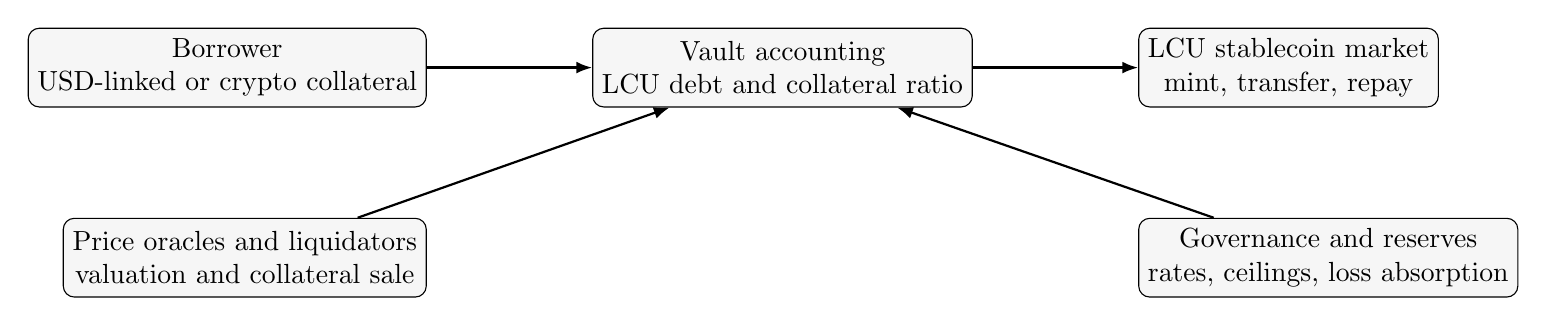
\begin{tikzpicture}[
node distance=1.4cm and 2.1cm,
box/.style={draw,rounded corners,align=center,minimum height=1.0cm,minimum width=3.1cm,fill=gray!7},
arr/.style={-{Latex[length=2mm]},thick}]
\node[box] (borrower) {Borrower\\USD-linked or crypto collateral};
\node[box,right=of borrower] (vault) {Vault accounting\\LCU debt and collateral ratio};
\node[box,right=of vault] (token) {LCU stablecoin market\\mint, transfer, repay};
\node[box,below left=of vault] (liquidator) {Price oracles and liquidators\\valuation and collateral sale};
\node[box,below right=of vault] (governance) {Governance and reserves\\rates, ceilings, loss absorption};
\draw[arr] (borrower) -- (vault);
\draw[arr] (vault) -- (token);
\draw[arr] (liquidator) -- (vault);
\draw[arr] (governance) -- (vault);
\end{tikzpicture}%
}
\caption{Minimal system context for the counterfactual local-currency vault. The empirical analysis evaluates the borrower's USD-equivalent liability; it does not implement these contracts.}\label{fig:architecture}
\end{figure*}

Let $P_i$ be the USD value of event $i$ at origination, and let $E_{i,0}$ and $E_{i,h}$ denote LCU per USD at origination and repayment horizon $h$. The hypothetical nominal debt issued at origination is $L_i=P_iE_{i,0}$. With no financing cost, its repayment value in USD is $L_i/E_{i,h}=P_iE_{i,0}/E_{i,h}$. Gross FX-driven debt erosion is therefore
\begin{equation}
B^{G}_{i,h}=P_i\left(1-\frac{E_{i,0}}{E_{i,h}}\right), \qquad
b^{G}_{i,h}=1-\frac{E_{i,0}}{E_{i,h}}.
\label{eq:gross}
\end{equation}
The measure is positive when the local currency depreciates against the dollar. We call it a \emph{benefit} rather than profit because it excludes collateral opportunity cost, tax, market impact, and unobserved borrower behaviour.

\section{Data and Empirical Design}\label{sec:data}

\subsection{MakerDAO event data}

The on-chain source is the public replication archive accompanying Chaleenutthawut et al. \cite{Chaleenutthawut2024}. The archive contains 4,466,880 successful traces to the MakerDAO \texttt{Vat} core-accounting contract, extracted from Google BigQuery for 12 November 2019 through 31 July 2023. The published query selects the Vat address, excludes reverted calls, orders traces by block and transaction position, and omits top-level calls with null trace addresses. We decode documented \texttt{fold}, \texttt{frob}, \texttt{grab}, and \texttt{fork} call signatures \cite{MakerVatDocs}.

For collateral type ETH-A, a borrowing event is a successful \texttt{Vat.frob} call with positive signed \texttt{dart}; it can be a first debt draw or additional borrowing from an existing vault. It is not a vault-opening event and not necessarily a unique person. DAI debt change equals normalised debt change multiplied by the collateral type's accumulated \texttt{rate}. The \texttt{urn} is reported as a vault-level identifier; we do not equate it with a verified real-world borrower. Event records contain transaction hashes so individual observations can be audited.

\begin{table*}[t]
\caption{Dataset construction and descriptive statistics.}\label{tab:sample}
\centering
\small
\begin{threeparttable}
\begin{tabular}{lrr}
\toprule
\multicolumn{3}{l}{\textit{Panel A: Sample construction}} \\
Stage & Count & Share of raw (\%) \\
\midrule
Raw successful Vat call traces & 4,466,880 & 100.00 \\
Decoded ETH-A debt-changing events & 229,224 & 5.13 \\
Positive ETH-A \texttt{frob} debt draws & 137,426 & 3.08 \\
Excluded before 1 January 2020 & 6,527 & 0.15 \\
Excluded below 1 DAI after date filter & 157 & $<0.01$ \\
Final debt-draw event sample & 130,742 & 2.93 \\
\midrule
\multicolumn{3}{l}{\textit{Panel B: Final event-sample description}} \\
Statistic & Value & Unit \\
\midrule
Unique ETH-A urn identifiers & 16,846 & vault identifiers \\
Verified unique borrower addresses & Not available & --- \\
Clean single-draw repaid lifecycles & 7,947 & reconstructed spells \\
Total positive debt change & 13.318 & billion DAI \\
Mean / median debt change & 101,865 / 4,792 & DAI \\
Standard deviation & 1,523,003 & DAI \\
Minimum / maximum & 1 / 150.450 & DAI / million DAI \\
Analysis dates & 2020-01-01--2023-07-31 & calendar dates \\
\bottomrule
\end{tabular}
\begin{tablenotes}[flushleft]\footnotesize
\item The \texttt{urn} field identifies a MakerDAO vault accounting position, not a verified person or necessarily the transaction sender. The public decoded files do not permit a defensible count of unique borrower-controlled addresses; that quantity is therefore reported as unavailable rather than inferred. The lifecycle count precedes FX-coverage filtering; 7,105 spells per currency enter the observed-duration robustness test.
\end{tablenotes}
\end{threeparttable}
\end{table*}

Table~\ref{tab:sample} replaces the former untraceable 1,000/981-event counts. The analysis window begins on 1 January 2020 and ends at the public archive boundary on 31 July 2023. Debt adjustments below 1 DAI are excluded as economically de minimis and to prevent fixed gas costs from creating near-singular percentage outcomes. The strong right skew motivates medians and amount-weighted estimates alongside unweighted means. No April 2026 repayment endpoint is used.

\subsection{Foreign-exchange data}

We use official monthly-average exchange rates from OECD Main Economic Indicators, distributed by the Federal Reserve Bank of St. Louis (FRED). The identifiers are \texttt{ARGCCUSMA02STM} for ARS per USD and \texttt{CCUSMA02TRM618N} for TRY per USD \cite{FREDARS,FREDTRY}. Both series are expressed as national-currency units per US dollar. Month $t+h$ is matched by calendar month; no interpolation is needed for eligible events. The data and source files are included in the replication package.

The ARS series is an official rate and may diverge from parallel-market rates under capital controls. Consequently, results describe the selected official-rate counterfactual, not the price at which every user could transact. As a timing robustness check, we combine adjacent months adversely for the borrower: the highest of $t-1,t,t+1$ is used at origination and the lowest of $t+h-1,t+h,t+h+1$ at repayment.

\begin{figure*}[t]
\centering
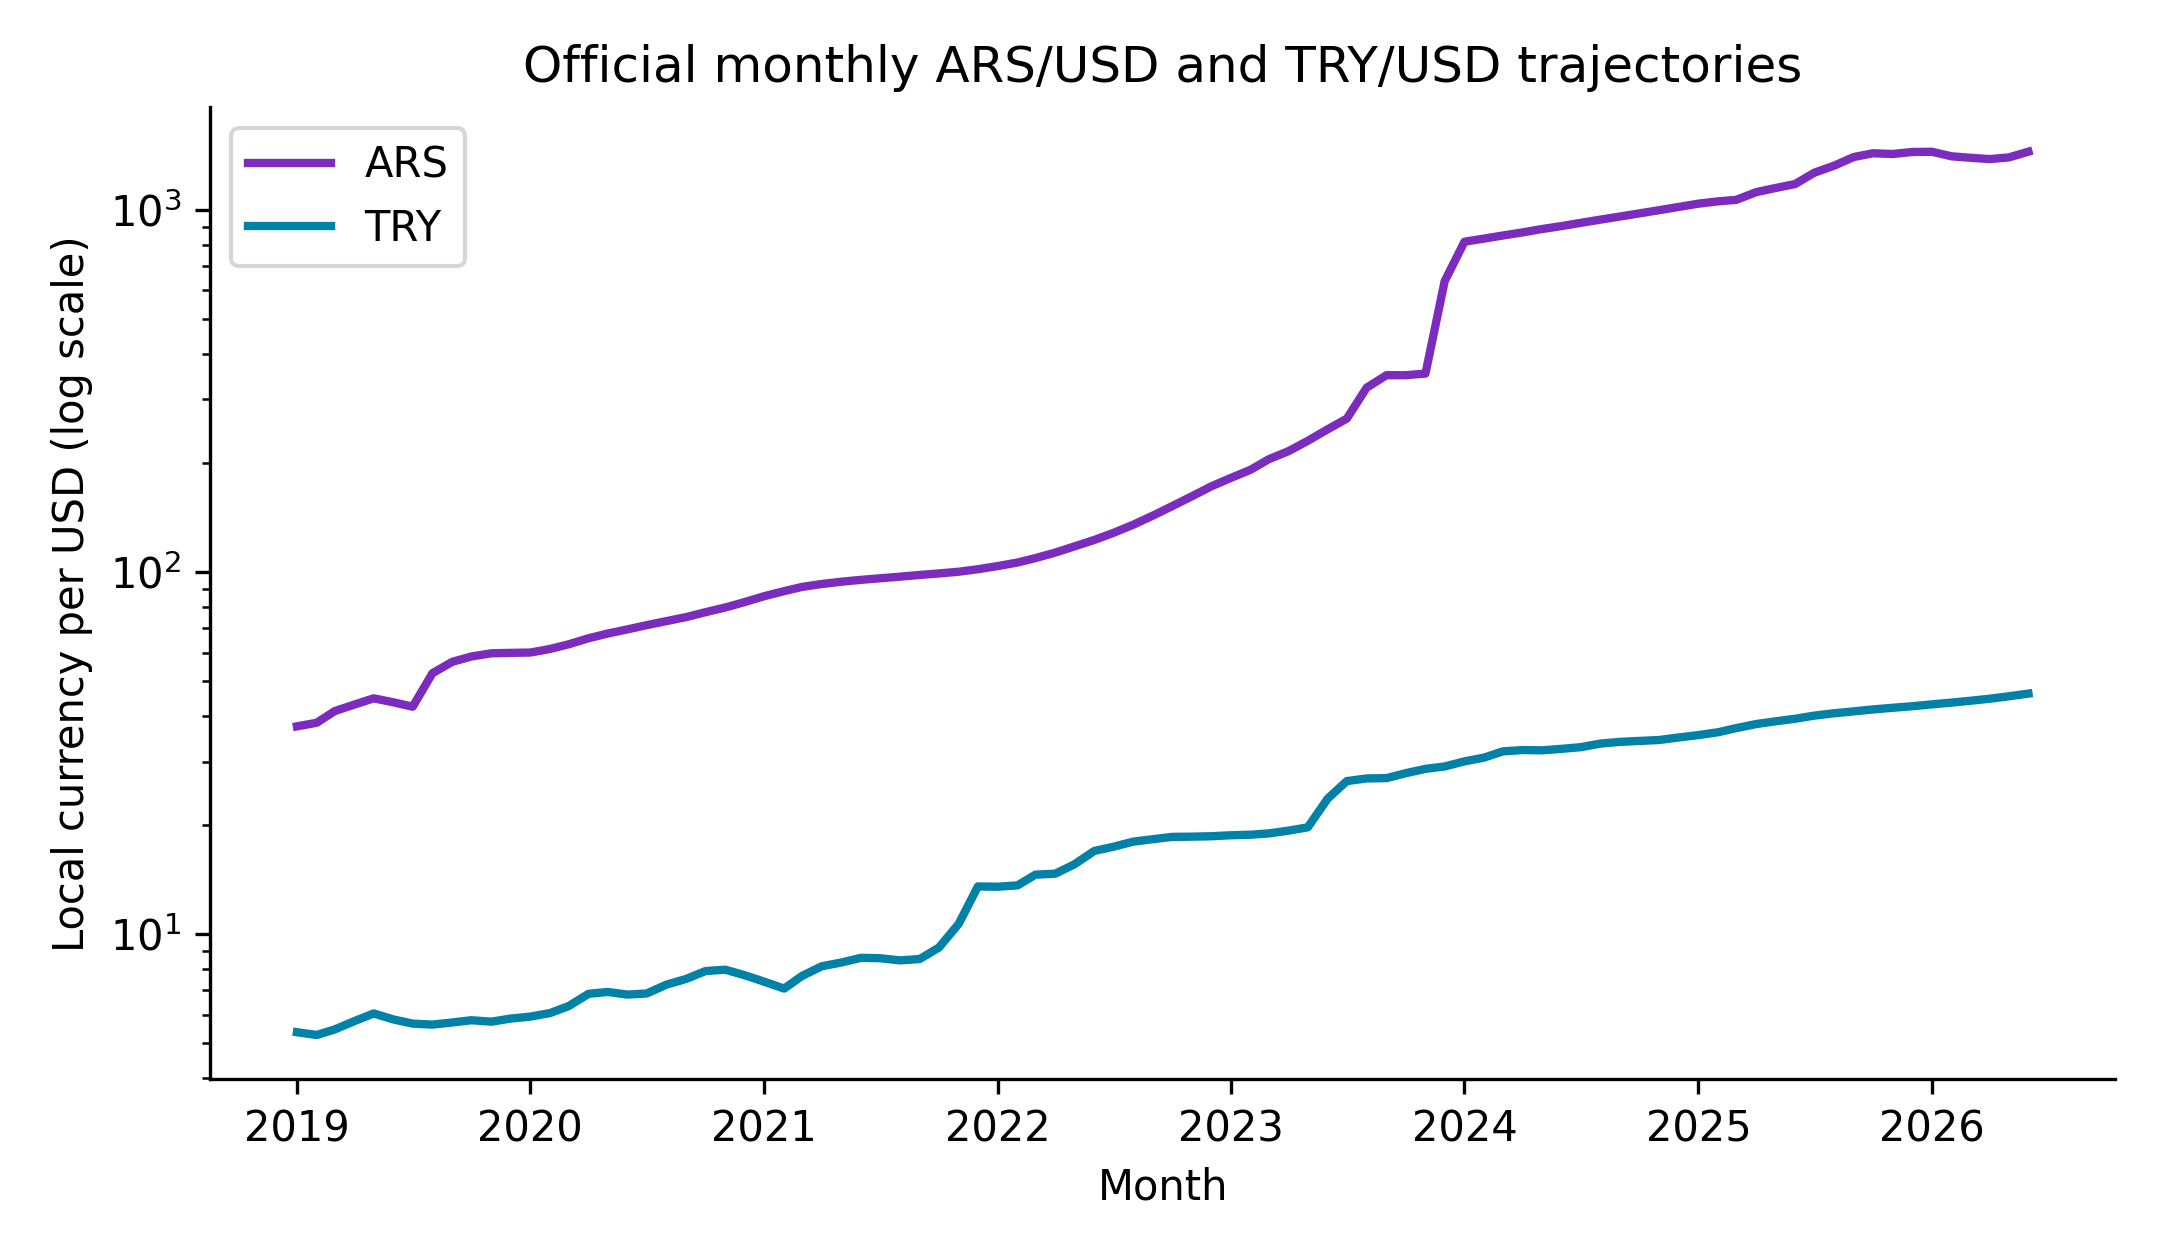
\includegraphics[width=0.78\textwidth]{figures/figure2.png}
\caption{Official monthly-average local-currency units per US dollar. The vertical axis is logarithmic. Source: OECD Main Economic Indicators via FRED.}\label{fig:fx}
\end{figure*}

\subsection{Fixed horizons, net benefits, and weighting}

Every event is evaluated at fixed 3-, 6-, 12-, and 24-month repayment horizons. This removes the former comparison of events with different terminal dates and ensures that $E_{i,0}=E_{i,h}$ mechanically yields zero gross benefit. Let $r$ be the annual borrowing rate, $T=h/12$, $f$ a protocol fee on discounted principal, $s$ the proportional conversion cost in each direction, and $g$ round-trip gas in USD. The model implemented in code is
\begin{align}
D_{i,h}(r) &= P_i\frac{E_{i,0}}{E_{i,h}}(1+r)^T,\\
C_{i,h} &= fP_i\frac{E_{i,0}}{E_{i,h}} + sP_i + sD_{i,h}(r) + g,\\
B^{N}_{i,h}(r) &= P_i-D_{i,h}(r)-C_{i,h}.
\label{eq:net}
\end{align}
The base case sets $f=0.5\%$, $s=0.3\%$ each way, $g=\$40$, and evaluates $r\in\{5,10,20,40,80,120\}\%$. Low and high execution-cost cases are $(f,s,g)=(0\%,0.1\%,\$10)$ and $(1\%,1\%,\$100)$. These are transparent scenarios, not estimates of a deployed local-currency protocol.

We report (i) the median event-level percentage, (ii) the share of event-position mappings with positive benefits, and (iii) an amount-weighted aggregate, $\sum_i B_i/\sum_iP_i$. The unweighted mean is also retained in the output files but is sensitive to fixed gas applied to small draws.

\begin{table*}[t]
\caption{Prespecified assumptions and scenario parameters.}\label{tab:assumptions}
\centering
\small
\begin{tabularx}{\textwidth}{p{3.1cm}p{5.0cm}X}
\toprule
Component & Values & Status or rationale \\
\midrule
Liability currencies & ARS and TRY & High-depreciation counterfactual cases \\
FX observations & Official monthly averages & OECD Main Economic Indicators via FRED \\
Fixed horizons & 3, 6, 12, and 24 months & Common calendar-month comparison \\
Annual borrowing rates & 5, 10, 20, 40, 80, and 120\% & Sensitivity grid; 20\% base case \\
Protocol / conversion fees & 0.5\%; 0.3\% in each direction & Base execution-cost scenario \\
Round-trip gas & USD 40 & Base execution-cost scenario \\
Collateral type & USD stablecoin, ETH, and BTC & Stable and volatile benchmarks \\
Initial / threshold ratio & 150, 175, 200\% / 150\% & Governance stress grid \\
Liquidation penalty & 5, 10, and 13\% of modeled debt & Sensitivity grid; 13\% base stress \\
Terminal crypto shock & 10, 25, 40, and 60\% & Static downside scenarios \\
Shock probabilities & 40, 30, 20, and 10\% & Illustrative weights; not empirically estimated \\
Near-liquidation buffer & 110\% of the threshold & Diagnostic status band \\
\bottomrule
\end{tabularx}
\begin{minipage}{0.96\textwidth}\footnotesize
\emph{Notes:} Parameters describe transparent scenarios rather than a calibrated, deployed ARS- or TRY-denominated protocol. All values are machine-readable in \texttt{results/assumptions\_parameters.csv}.
\end{minipage}
\end{table*}

\subsection{Lifecycle and collateral-risk robustness}

The archive excludes top-level calls. A complete historical debt path therefore cannot be guaranteed for every urn. We reconstruct spells and retain only internally consistent, single-draw, single-repayment, non-liquidated, non-forked lifecycles for the observed-duration robustness test. This is a restricted check, not a representative survival estimate.

The collateral screen evaluates a 12-month horizon at $r=20\%$. Initial collateral ratios are 150\%, 175\%, and 200\%; the liquidation threshold is 150\%; penalties are 5\%, 10\%, and 13\%; and terminal crypto-collateral shocks are 10\%, 25\%, 40\%, and 60\%. A USD-stablecoin collateral benchmark has a zero price shock. Let $q_s$ be the terminal collateral decline in scenario $s$, $\theta$ the liquidation threshold, $\lambda$ the penalty rate, and $CR_0$ the initial collateral ratio. The terminal status and penalty loss are
\begin{align}
I_{i,s} &= \mathbb{1}\!\left\{\frac{CR_0P_i(1-q_s)}{D_{i,12}(r)}<\theta\right\},\\
EL_i &= \sum_s p_s\lambda D_{i,12}(r)I_{i,s}, \qquad
B^R_i=B^N_{i,12}(r)-EL_i,
\label{eq:expectedloss}
\end{align}
where $p_s=(0.40,0.30,0.20,0.10)$ are illustrative rather than estimated probabilities. Each mapping is labelled \emph{healthy} when its terminal ratio is at least 110\% of the threshold, \emph{near liquidation} when it lies between the threshold and that buffer, and \emph{liquidated} when it breaches the threshold. The screen is deliberately static and does not model within-horizon price paths, auction slippage, or oracle latency.

\section{Results}\label{sec:results}

\subsection{Borrowing-event distribution}

The final sample represents 13.318 billion DAI of positive ETH-A debt changes. Event sizes are highly right-skewed: the median is 4,792 DAI, the mean is 101,865 DAI, and the maximum is 150.45 million DAI (Table~\ref{tab:sample}). Figure~\ref{fig:distribution} shows why results should not be summarised with one unweighted mean.

\begin{figure*}[t]
\centering
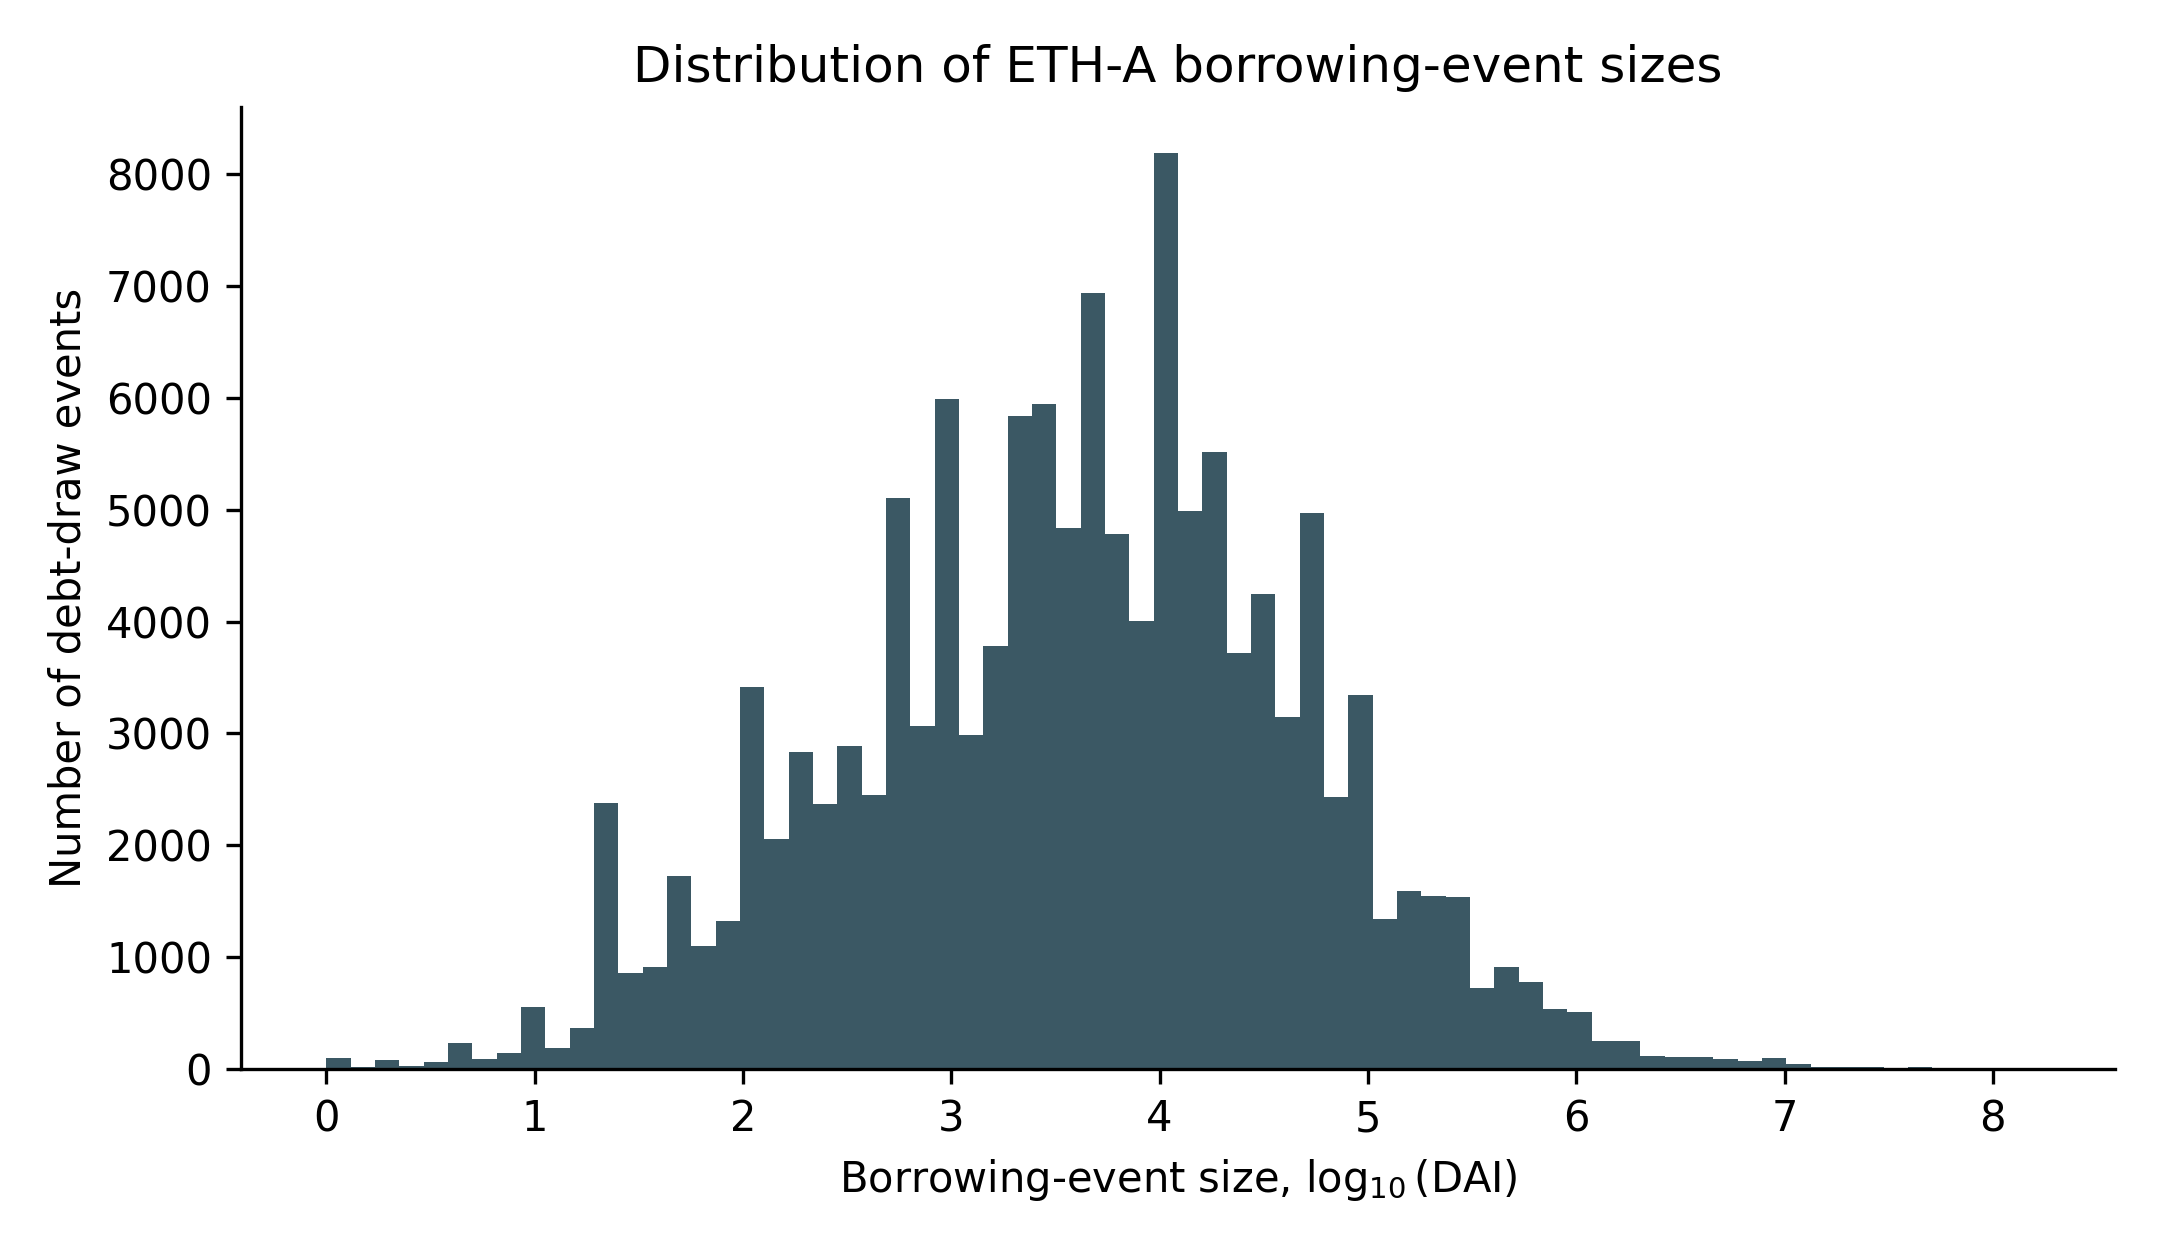
\includegraphics[width=0.7\textwidth]{figures/figure3.png}
\caption{Distribution of event sizes after the 1 DAI threshold.}\label{fig:distribution}
\end{figure*}

Figure~\ref{fig:activity} separates the number of draws from their total value. The two series need not move together because a small number of large events can dominate aggregate DAI volume.

\begin{figure*}[t]
\centering
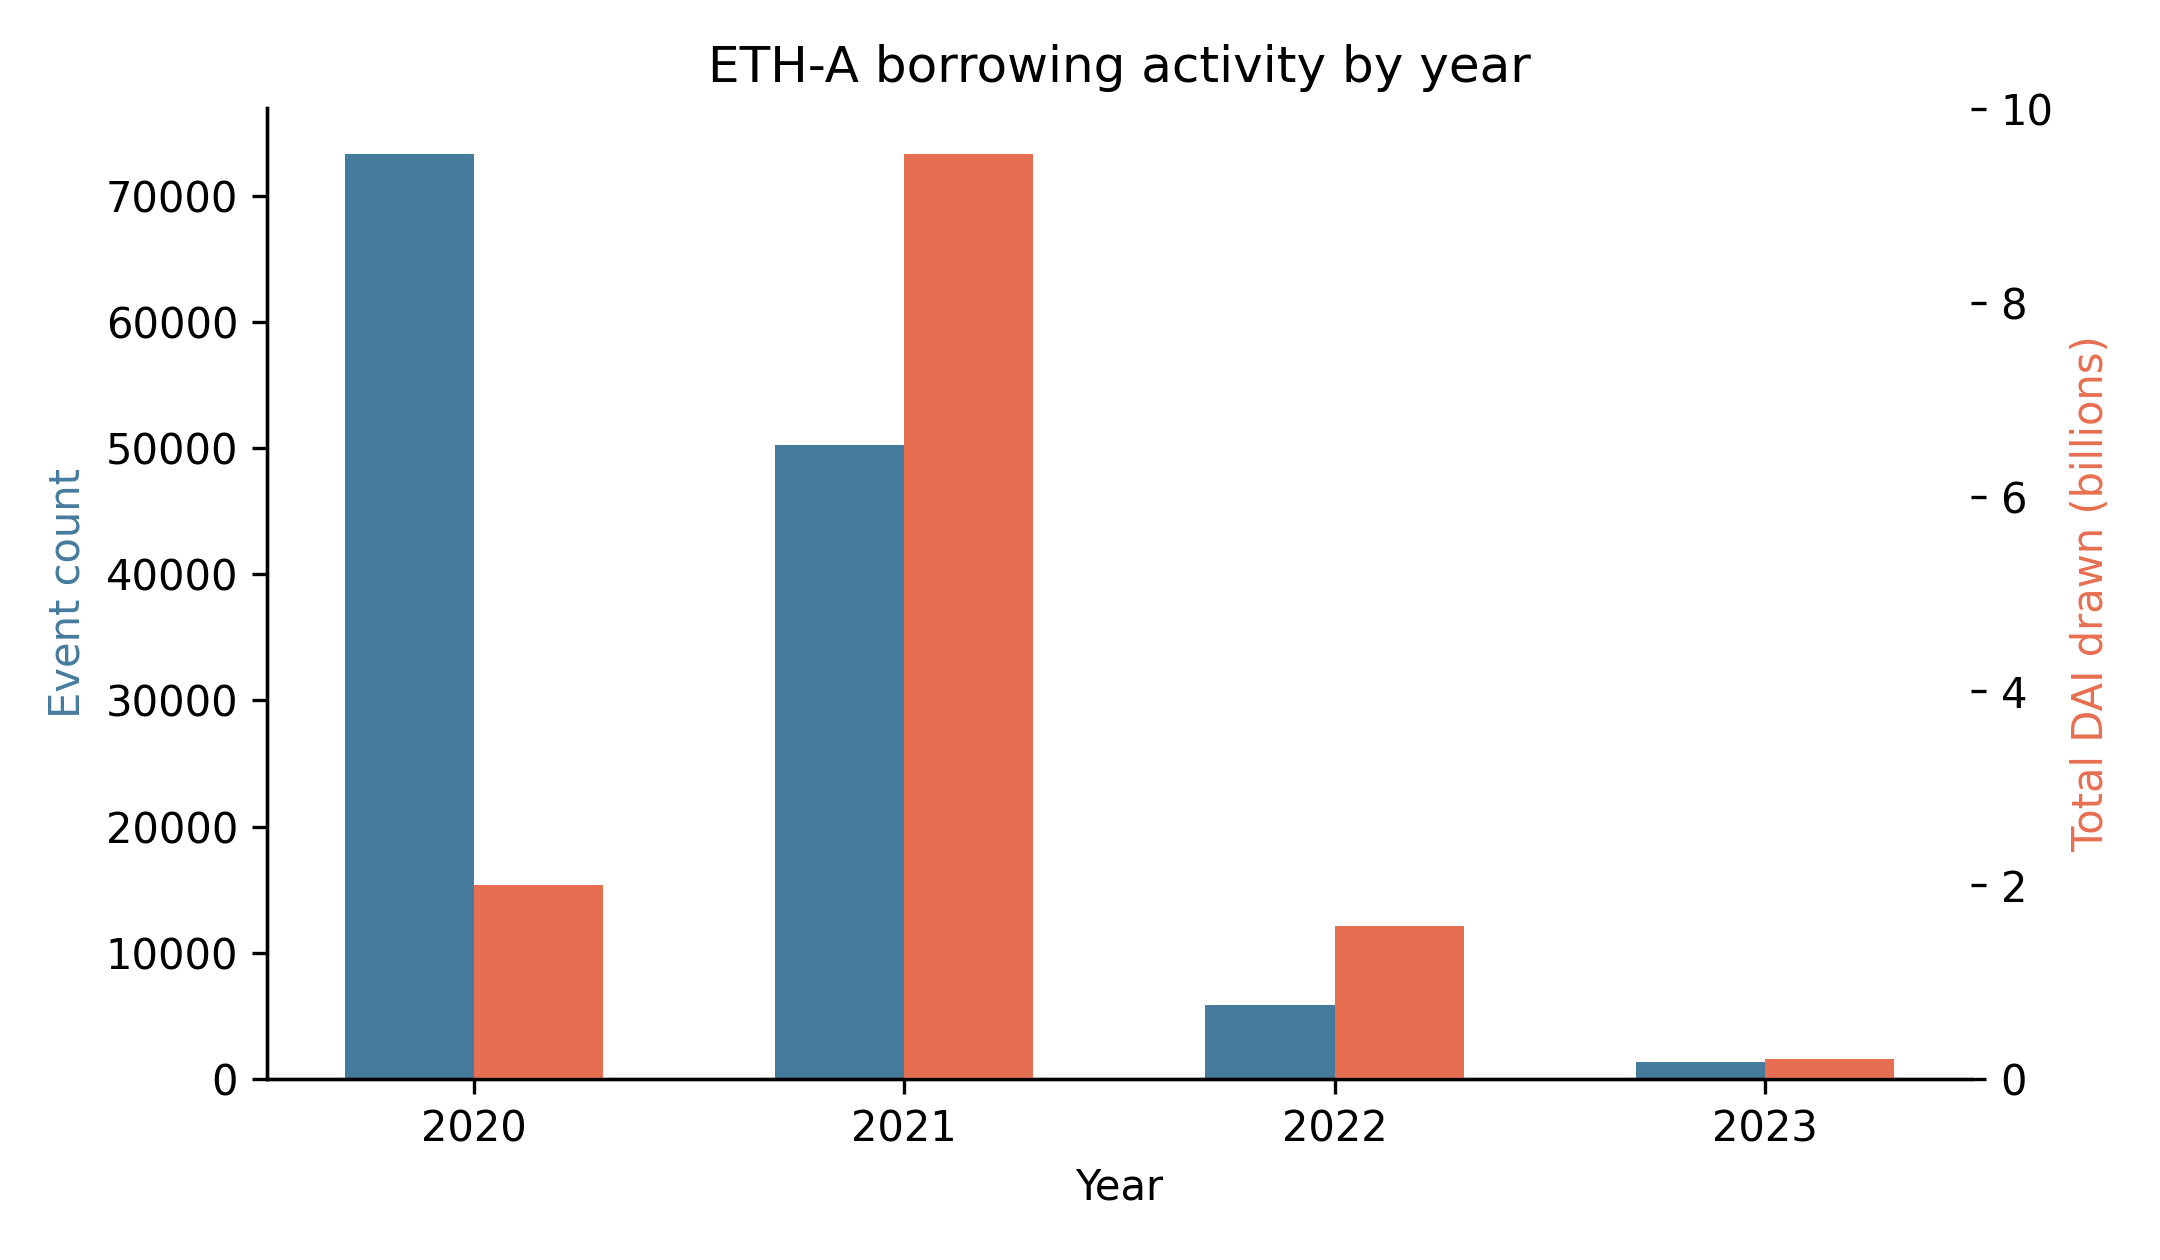
\includegraphics[width=0.82\textwidth]{figures/figure4.png}
\caption{Annual ETH-A borrowing activity in the final sample: event count and total positive debt change. The 2023 bar covers January through July.}\label{fig:activity}
\end{figure*}

\subsection{Gross FX-driven debt erosion (RQ1)}

\begin{table*}[t]
\caption{Gross FX-driven debt-erosion benefit by fixed horizon.}\label{tab:gross}
\centering
\small
\resizebox{\textwidth}{!}{%
\begin{tabular}{lrrrrrrrrr}
\toprule
Currency & Horizon & Events & Total DAI (bn) & Mean (\%) & Median (\%) & SD (pp) & IQR (pp) & Positive (\%) & Weighted (\%) \\
\midrule
ARS & 3 months  & 130,742 & 13.318 & 7.52 & 7.91 & 2.85 & 3.25 & 100.00 & 6.26 \\
ARS & 6 months  & 130,742 & 13.318 & 13.91 & 15.28 & 5.59 & 6.06 & 100.00 & 12.69 \\
ARS & 12 months & 130,742 & 13.318 & 26.03 & 24.61 & 9.23 & 11.26 & 100.00 & 28.11 \\
ARS & 24 months & 130,742 & 13.318 & 52.72 & 50.72 & 11.71 & 14.50 & 100.00 & 63.67 \\
TRY & 3 months  & 130,742 & 13.318 & 7.71 & 9.06 & 8.81 & 10.23 & 86.42 & 12.40 \\
TRY & 6 months  & 130,742 & 13.318 & 14.42 & 13.68 & 9.71 & 6.35 & 94.63 & 21.50 \\
TRY & 12 months & 130,742 & 13.318 & 30.40 & 25.30 & 14.63 & 28.30 & 100.00 & 40.83 \\
TRY & 24 months & 130,742 & 13.318 & 58.46 & 57.78 & 3.99 & 4.39 & 100.00 & 60.22 \\
\bottomrule
\end{tabular}
}
\begin{minipage}{0.94\textwidth}\footnotesize
\emph{Notes:} Gross benefit is $100(1-E_0/E_h)$. It excludes rates, fees, transaction costs, liquidation, tax, and collateral opportunity cost. ``Positive'' is the percentage of event-position mappings above zero.
\end{minipage}
\end{table*}

Table~\ref{tab:gross} and Figure~\ref{fig:gross} answer RQ1. The median gross effect rises monotonically with horizon, from 7.91\% to 50.72\% for ARS and from 9.06\% to 57.78\% for TRY. At 12 months the medians are similar, but the TRY distribution has a higher amount-weighted effect. These are consequences of historical event timing and official FX paths, not observed MakerDAO borrower gains.

\begin{figure*}[t]
\centering
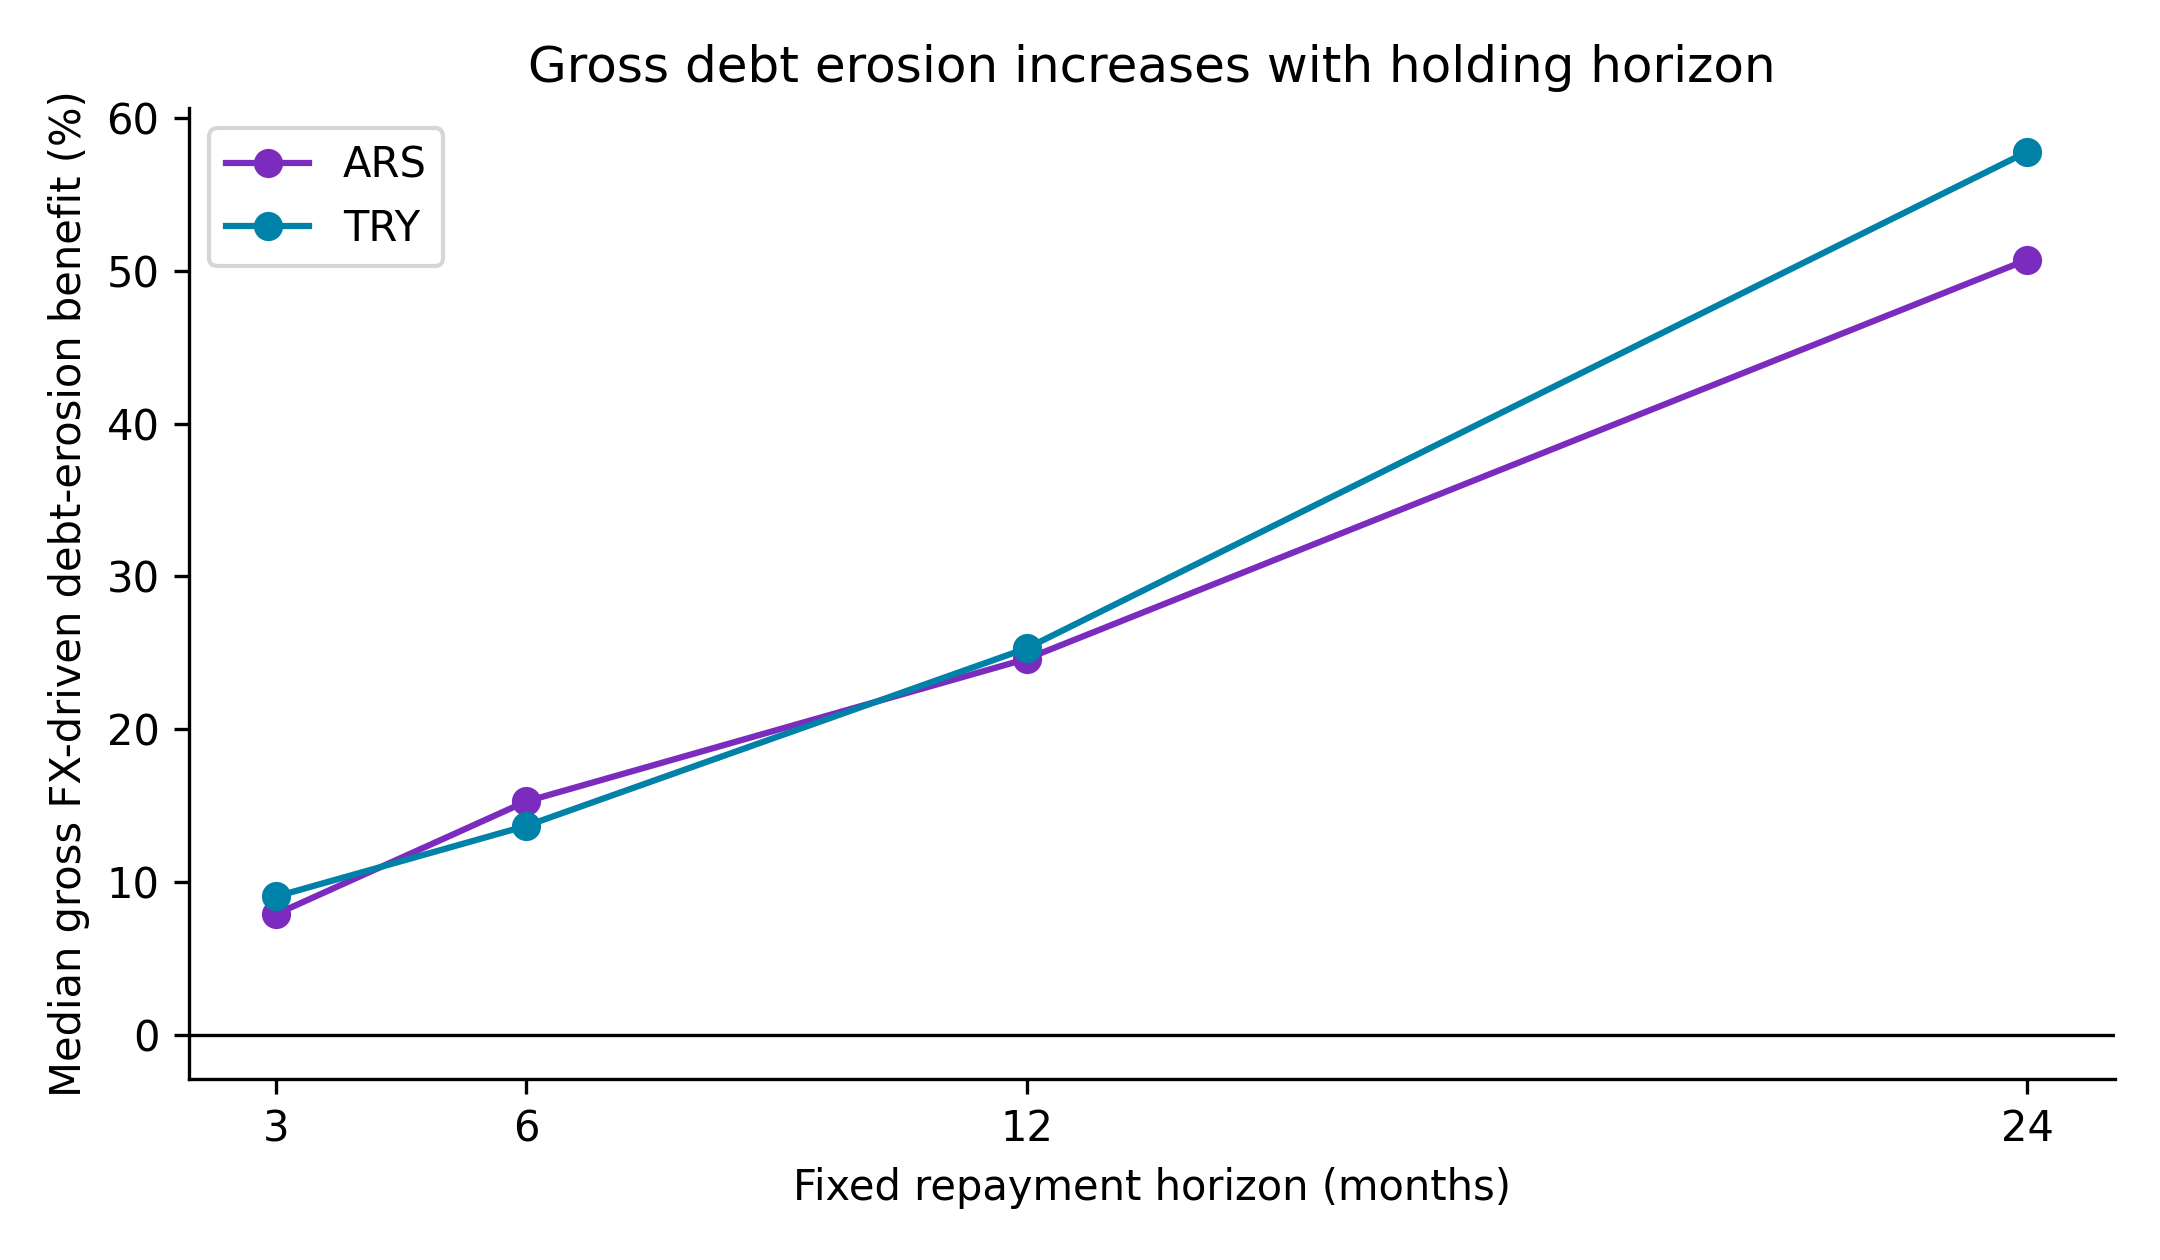
\includegraphics[width=0.7\textwidth]{figures/figure5.png}
\caption{Median gross FX-driven debt erosion at prespecified horizons.}\label{fig:gross}
\end{figure*}

\subsection{Financing and execution costs (RQ2)}

\begin{table*}[t]
\caption{Twelve-month pre-liquidation net benefit under rate sensitivity.}\label{tab:net}
\centering
\small
\begin{tabular}{lrrrrrrrr}
\toprule
& \multicolumn{4}{c}{ARS} & \multicolumn{4}{c}{TRY} \\
\cmidrule(lr){2-5}\cmidrule(lr){6-9}
Rate & Mean & Median & Positive & Weighted & Mean & Median & Positive & Weighted \\
(\%) & (\%) & (\%) & (\%) & (\%) & (\%) & (\%) & (\%) & (\%) \\
\midrule
5   & -0.59 & 14.60 & 87.57 & 23.60 & 4.04 & 18.19 & 82.64 & 37.05 \\
10  & -4.30 & 10.74 & 86.26 & 19.99 & 0.55 & 14.36 & 78.33 & 34.09 \\
20  & -11.72 & 2.78 & 62.05 & 12.78 & -6.43 & 6.71 & 57.27 & 28.15 \\
40  & -26.56 & -13.02 & 15.11 & -1.64 & -20.39 & -8.64 & 43.66 & 16.28 \\
80  & -56.24 & -44.92 & 4.05 & -30.48 & -48.31 & -38.62 & 28.06 & -7.45 \\
120 & -85.91 & -76.89 & 1.75 & -59.32 & -76.23 & -68.73 & 0.00 & -31.19 \\
\bottomrule
\end{tabular}
\begin{minipage}{0.94\textwidth}\footnotesize
\emph{Notes:} Base costs are a 0.5\% protocol fee, 0.3\% conversion cost each way, and USD 40 round-trip gas. Weighted is $100\sum_i B_i^N/\sum_iP_i$.
\end{minipage}
\end{table*}

At the base 20\% rate, median effects remain positive but much smaller: 2.78\% for ARS and 6.71\% for TRY (Table~\ref{tab:net}). Only 62.05\% and 57.27\% of event-position mappings, respectively, are positive. The negative unweighted means reflect fixed gas applied to many small events, whereas amount-weighted benefits remain 12.78\% and 28.15\%. At 40\%, both medians are negative. The median 12-month break-even annual rates are 23.85\% for ARS and 31.90\% for TRY; the full distributions are reported in the replication files.

Execution costs also alter classification. At a 20\% rate, the low/base/high cost scenarios produce ARS medians of 6.49\%, 2.78\%, and $-1.57$\%, with positive shares of 82.45\%, 62.05\%, and 43.45\%. TRY medians are 9.17\%, 6.71\%, and 2.40\%, with positive shares of 64.00\%, 57.27\%, and 52.94\%. RQ2 therefore has a conditional answer: depreciation can exceed modeled costs, but the result is not robust to all rates, position sizes, and execution assumptions.

\begin{figure*}[t]
\centering
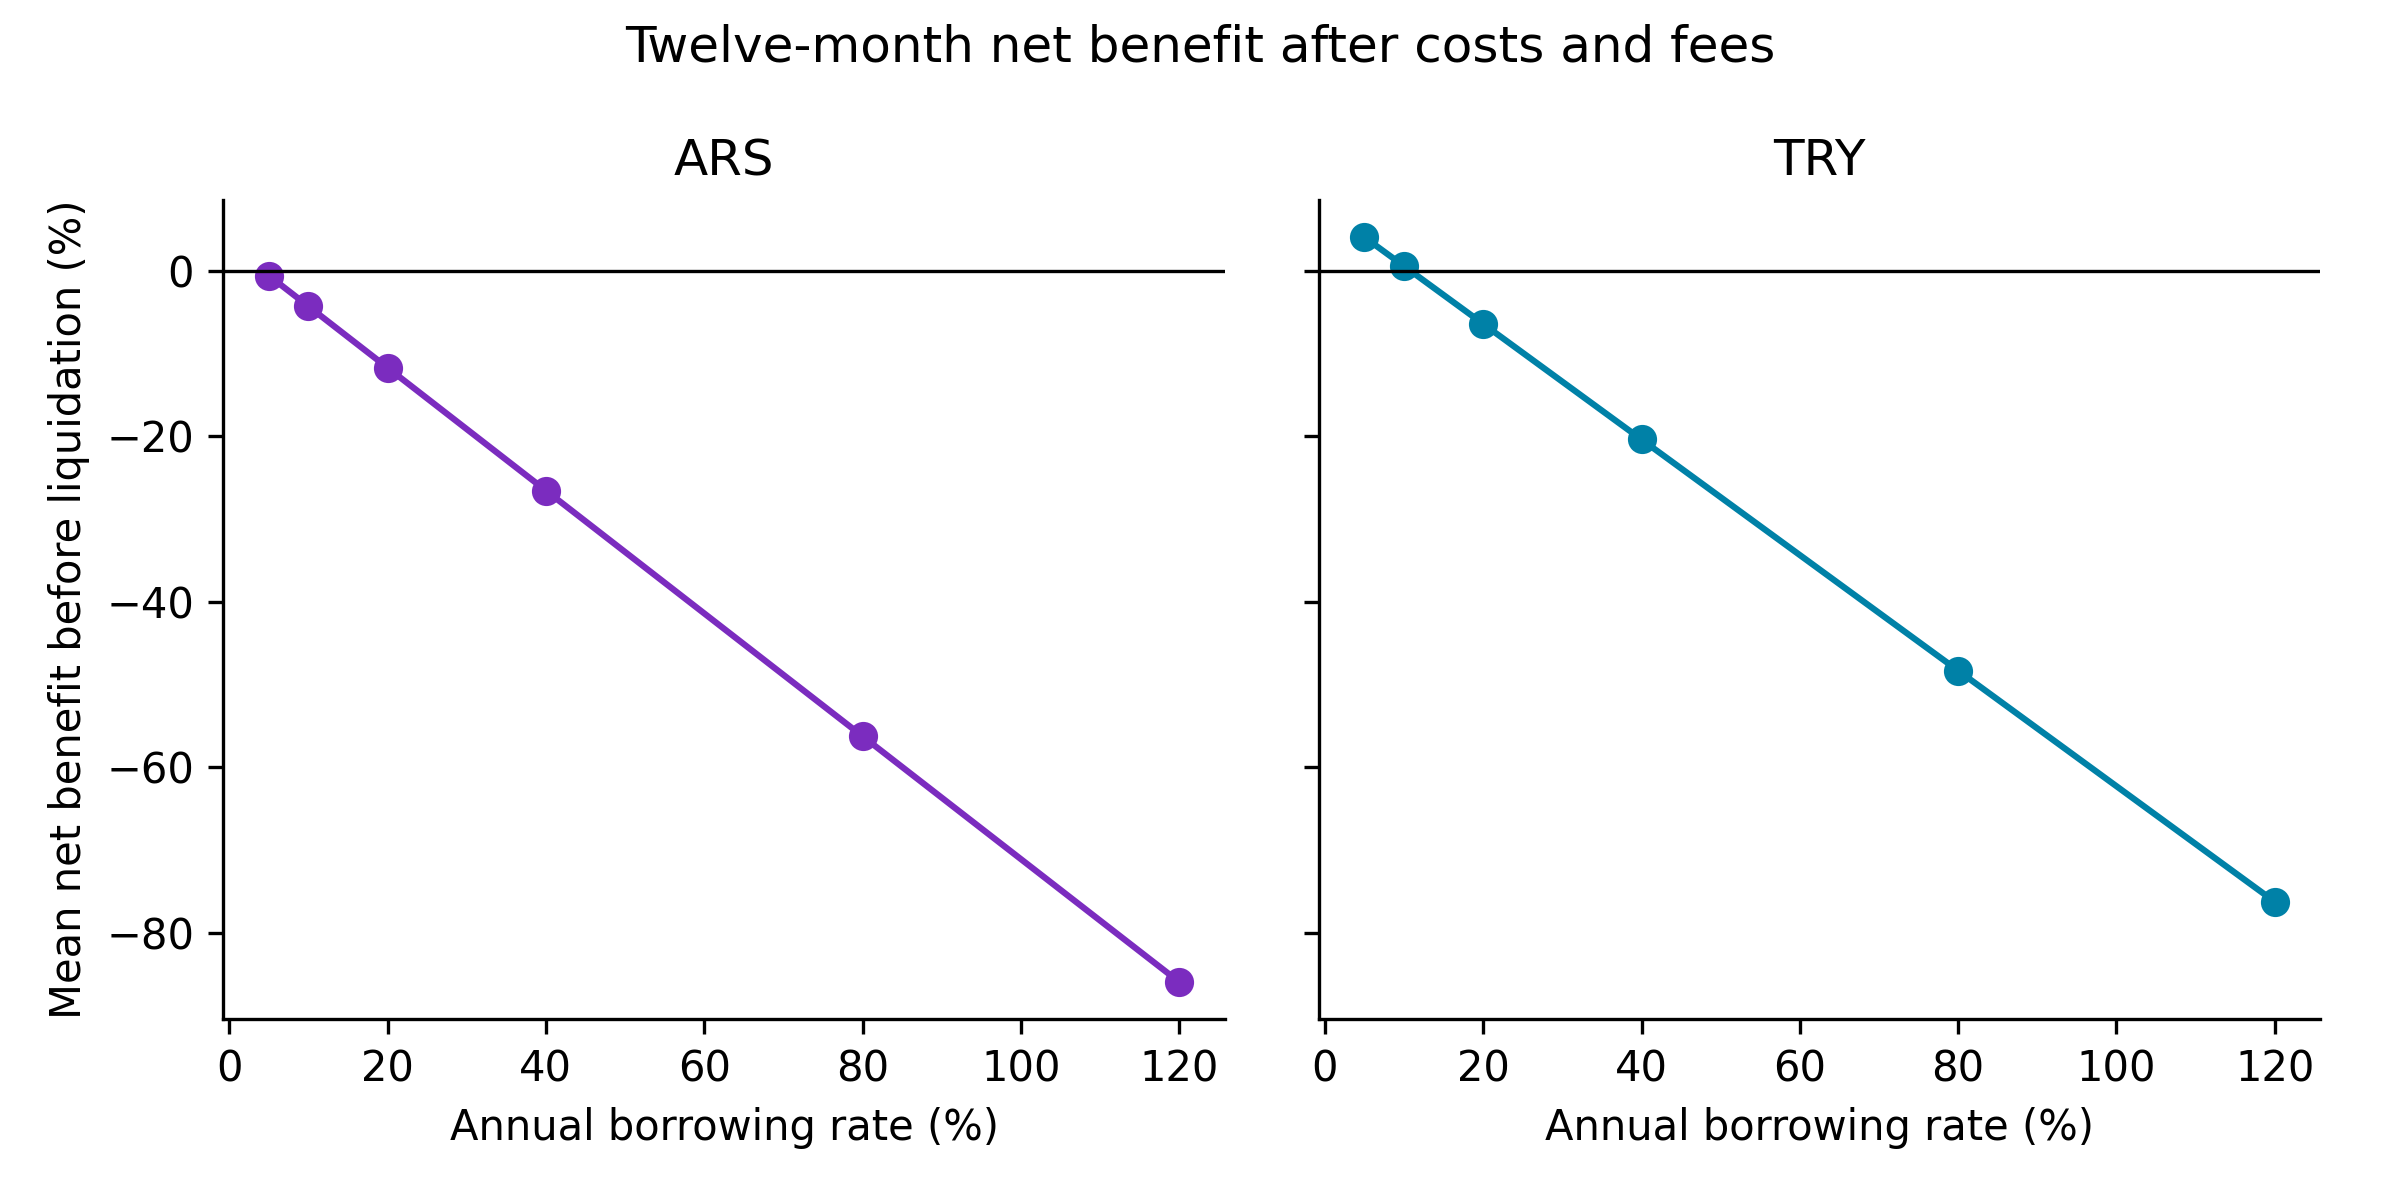
\includegraphics[width=0.78\textwidth]{figures/figure6.png}
\caption{Unweighted mean twelve-month net benefit before liquidation under borrowing-rate sensitivity. Fixed gas makes the mean especially conservative for small debt draws.}\label{fig:net}
\end{figure*}

\begin{figure*}[t]
\centering
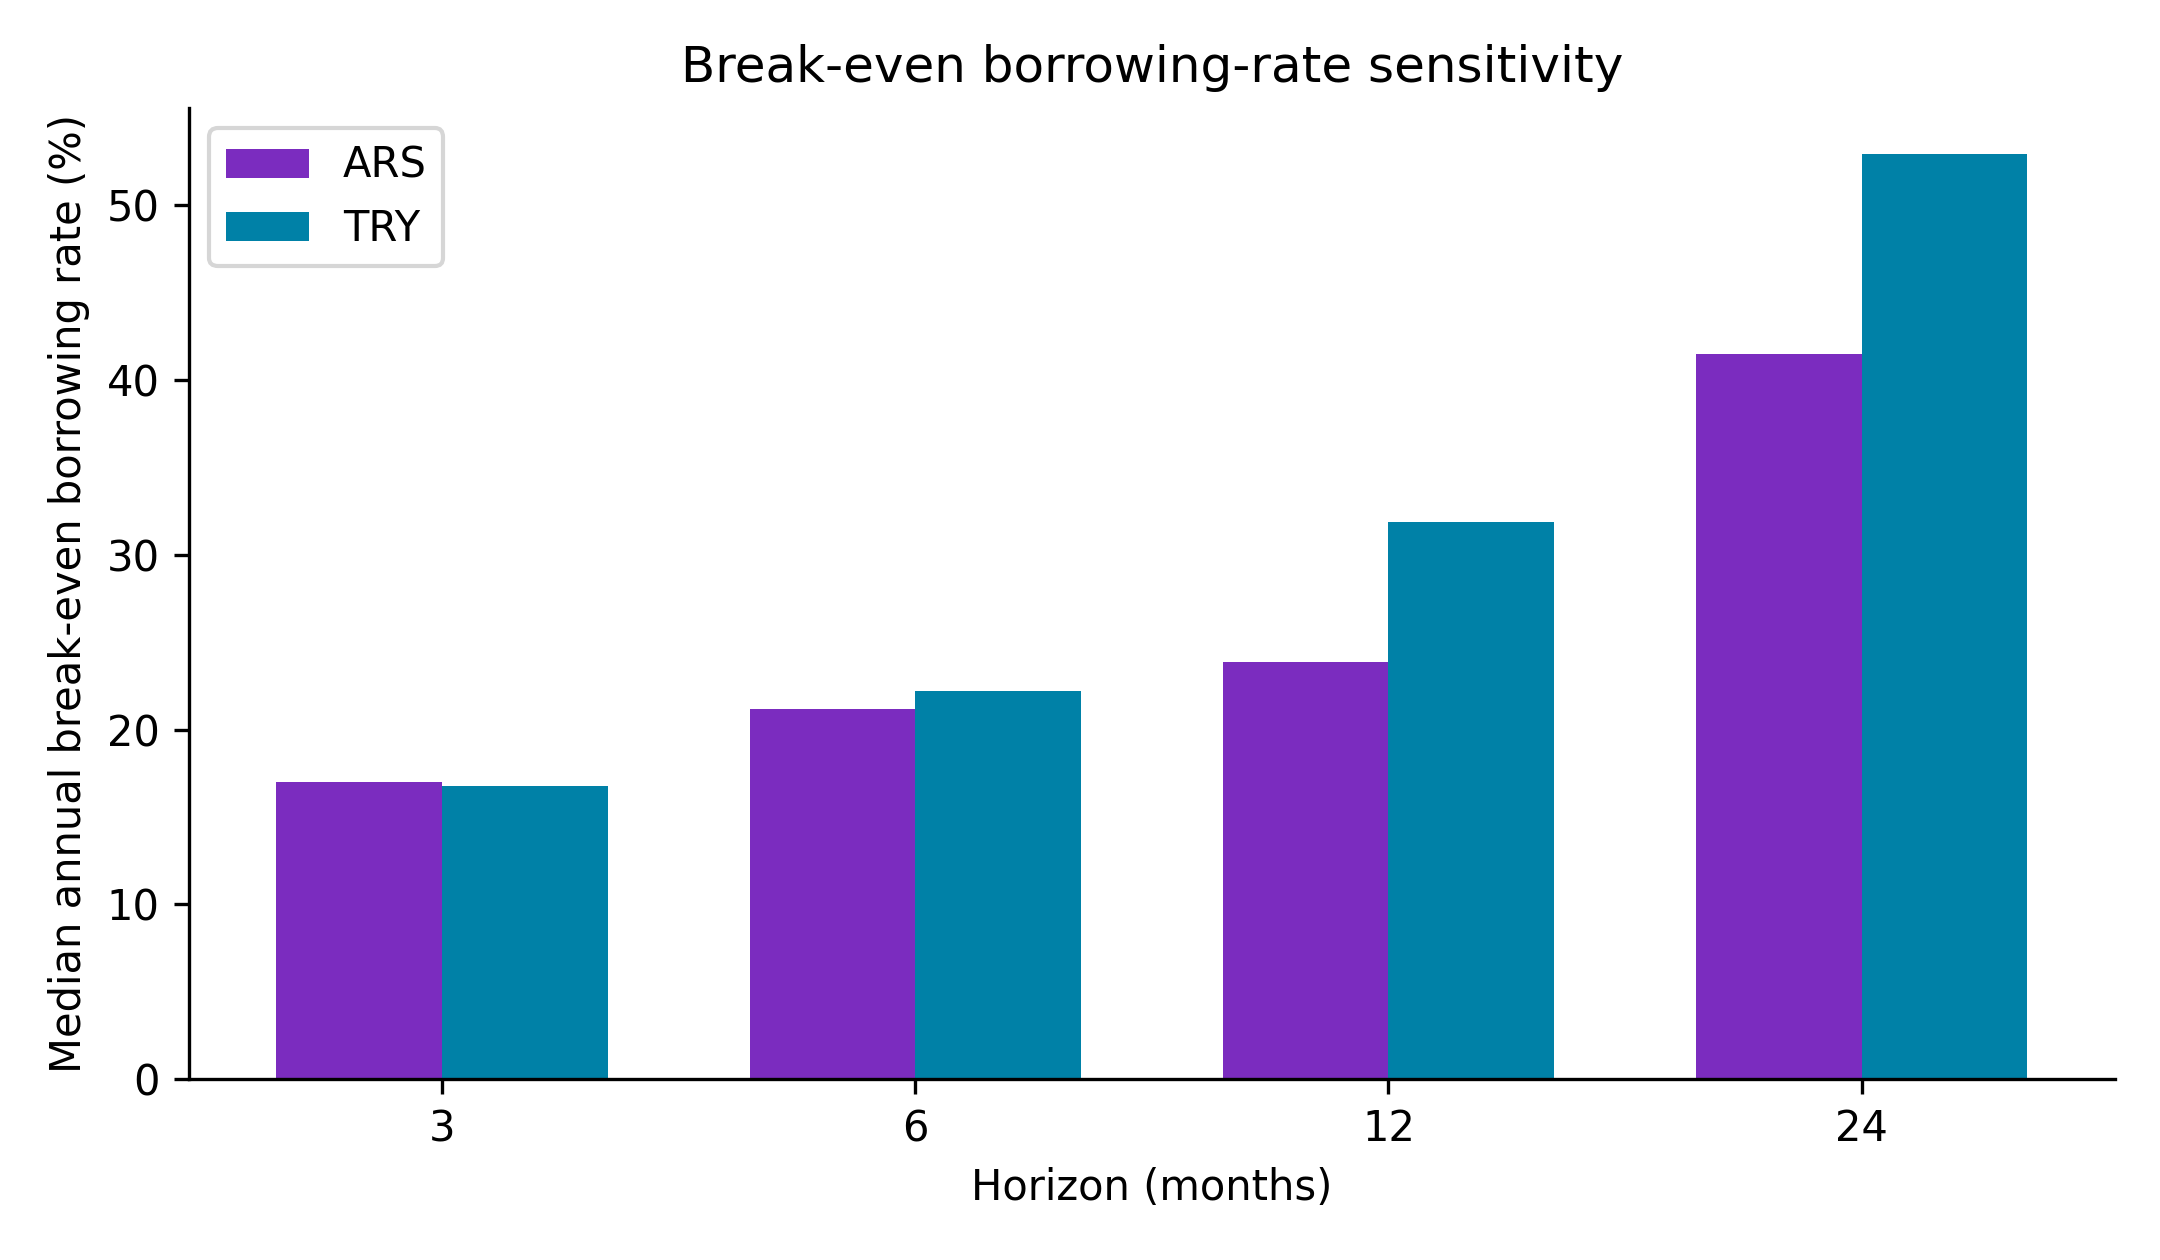
\includegraphics[width=0.76\textwidth]{figures/figure7.png}
\caption{Median annual break-even borrowing rate by fixed repayment horizon under base execution costs.}\label{fig:breakeven}
\end{figure*}

\subsection{Collateral stress (RQ3)}

\begin{table*}[t]
\caption{Collateral stress and scenario-weighted expected-loss results.}\label{tab:stress}
\centering
\scriptsize
\resizebox{\textwidth}{!}{%
\begin{tabular}{llrrrrrr}
\toprule
\multicolumn{8}{l}{\textit{Panel A: Terminal breach share by initial collateral ratio and crypto shock}} \\
Currency & Collateral & Initial ratio & 10\% shock & 25\% shock & 40\% shock & 60\% shock & Threshold \\
\midrule
ARS & ETH/BTC & 150\% & 50.42 & 92.33 & 97.30 & 98.87 & 150\% \\
ARS & ETH/BTC & 175\% & 0.00 & 59.92 & 94.48 & 98.87 & 150\% \\
ARS & ETH/BTC & 200\% & 0.00 & 5.24 & 90.55 & 98.20 & 150\% \\
TRY & ETH/BTC & 150\% & 48.50 & 57.68 & 93.42 & 100.00 & 150\% \\
TRY & ETH/BTC & 175\% & 3.76 & 53.41 & 58.29 & 100.00 & 150\% \\
TRY & ETH/BTC & 200\% & 0.00 & 24.67 & 56.78 & 100.00 & 150\% \\
\midrule
\multicolumn{8}{l}{\textit{Panel B: Scenario-weighted expected loss at a 175\% initial ratio}} \\
Currency & Collateral & Penalty & Expected breach & Expected loss & Median risk-adjusted & Positive & Weighted \\
& & (\%) & probability (\%) & (\% of principal) & benefit (\%) & (\%) & benefit (\%) \\
\midrule
ARS & USD stablecoin & 13 & 0.00 & 0.00 & 2.78 & 62.05 & 12.78 \\
ARS & ETH/BTC & 5 & 46.76 & 2.15 & 0.06 & 50.45 & 10.74 \\
ARS & ETH/BTC & 10 & 46.76 & 4.31 & -2.73 & 40.36 & 8.71 \\
ARS & ETH/BTC & 13 & 46.76 & 5.60 & -4.44 & 35.56 & 7.49 \\
TRY & USD stablecoin & 13 & 0.00 & 0.00 & 6.71 & 57.27 & 28.15 \\
TRY & ETH/BTC & 5 & 39.18 & 1.86 & 3.95 & 53.11 & 27.22 \\
TRY & ETH/BTC & 10 & 39.18 & 3.72 & 1.19 & 51.09 & 26.28 \\
TRY & ETH/BTC & 13 & 39.18 & 4.84 & -0.47 & 49.76 & 25.72 \\
\bottomrule
\end{tabular}
}
\begin{minipage}{0.96\textwidth}\footnotesize
\emph{Notes:} Panel A reports percentages of event-position mappings. ETH and BTC coincide because the screen applies the same percentage shock rather than asset-specific return distributions. A zero-shock USD-stablecoin benchmark has no breach at the 175\% ratio. Panel B weights the 10/25/40/60\% shocks by 40/30/20/10\%. The probabilities are illustrative, not estimated. Expected loss includes the indicated liquidation penalty but excludes auction slippage and path dependence.
\end{minipage}
\end{table*}

Crypto-collateral declines can dominate the FX benefit. At a 175\% initial ratio, a 25\% decline causes 59.92\% of ARS mappings and 53.41\% of TRY mappings to breach the screen (Table~\ref{tab:stress}, Panel A). Under the illustrative shock weights and a 13\% penalty, median risk-adjusted benefits fall from 2.78\% to $-4.44$\% for ARS and from 6.71\% to $-0.47$\% for TRY (Panel B). The corresponding expected losses are 5.60\% and 4.84\% of principal. A stablecoin-collateral benchmark has no shock-triggered liquidation at the 175\% ratio, although it retains issuer, depeg, and custody risks. Thus RQ3 is conditional: debt erosion may be material before liquidation, but crypto-collateral stress sharply reduces its reliability.

\begin{figure*}[t]
\centering
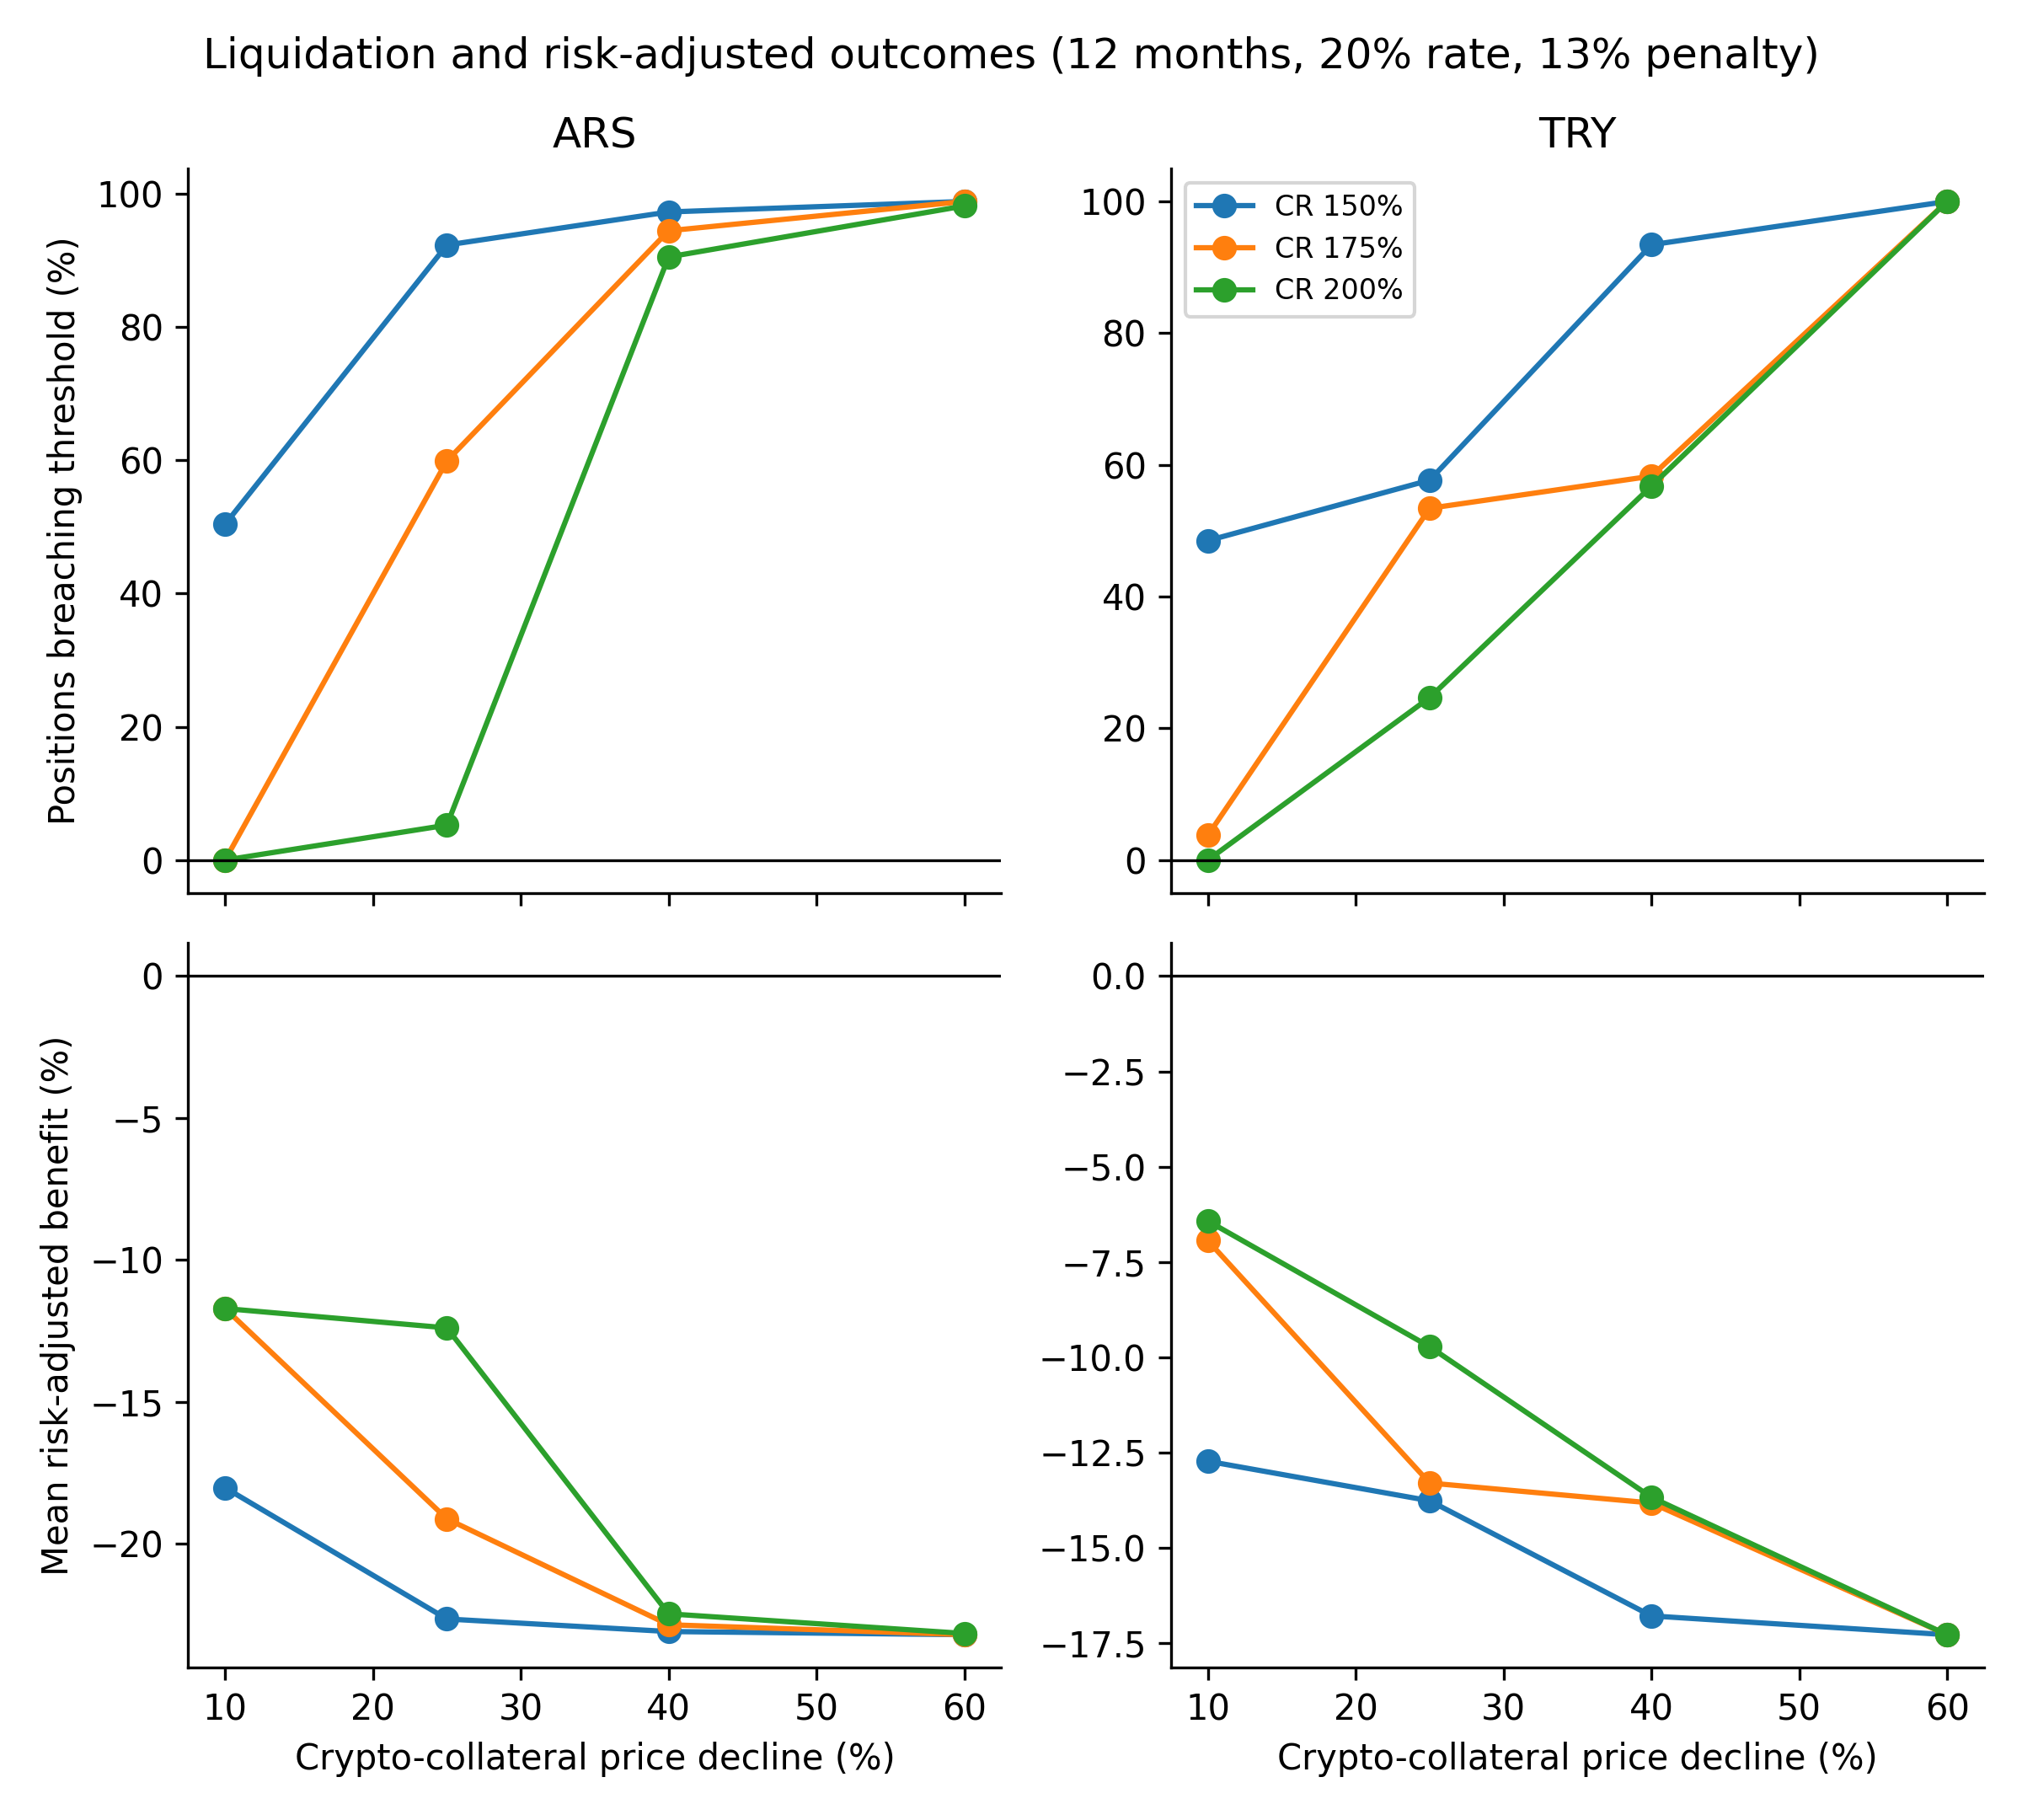
\includegraphics[width=0.92\textwidth]{figures/figure8.png}
\caption{Collateral-stress diagnostics. Top panels show terminal breach shares across crypto shocks and initial collateral ratios; bottom panels show mean risk-adjusted benefits within each terminal-shock scenario.}\label{fig:liquidation}
\end{figure*}

\subsection{Robustness checks}

\begin{table*}[t]
\caption{Robustness and execution-cost checks.}\label{tab:robustness}
\centering
\scriptsize
\resizebox{\textwidth}{!}{%
\begin{tabular}{llp{4.3cm}rrrr}
\toprule
Test & Currency & Specification & Events/spells & Median (\%) & Positive (\%) & Weighted (\%) \\
\midrule
FX timing & ARS & Adjacent-month conservative gross & 130,742 & 21.85 & 100.00 & --- \\
FX timing & TRY & Adjacent-month conservative gross & 130,742 & 17.05 & 100.00 & --- \\
Observed duration & ARS & Lifecycle net, 20\% rate/base costs & 7,105 & -2.99 & 13.19 & --- \\
Observed duration & TRY & Lifecycle net, 20\% rate/base costs & 7,105 & -4.13 & 14.58 & --- \\
Execution cost & ARS & Low cost & 130,742 & 6.49 & 82.45 & 13.54 \\
Execution cost & ARS & Base cost & 130,742 & 2.78 & 62.05 & 12.78 \\
Execution cost & ARS & High cost & 130,742 & -1.57 & 43.45 & 11.06 \\
Execution cost & TRY & Low cost & 130,742 & 9.17 & 64.00 & 28.82 \\
Execution cost & TRY & Base cost & 130,742 & 6.71 & 57.27 & 28.15 \\
Execution cost & TRY & High cost & 130,742 & 2.40 & 52.94 & 26.60 \\
\bottomrule
\end{tabular}
}
\begin{minipage}{0.96\textwidth}\footnotesize
\emph{Notes:} The FX-timing rows report gross benefits; all other rows report pre-liquidation net benefits. The lifecycle subset comprises internally consistent single-draw, single-repayment, non-liquidated, non-forked spells with FX coverage. Low/base/high costs are defined in Table~\ref{tab:assumptions}.
\end{minipage}
\end{table*}

The conservative adjacent-month FX match reduces the 12-month median gross effect from 24.61\% to 21.85\% for ARS and from 25.30\% to 17.05\% for TRY; all matched positions remain positive in this historical window (Table~\ref{tab:robustness}). This check addresses monthly timing, not the official-versus-parallel-market distinction.

The clean lifecycle check contains 7,105 spells with FX coverage in each currency and a median duration of 6.95 days. Its median gross effect is zero because many spells begin and end in the same monthly observation. At a 20\% rate and base costs, median net benefits are $-2.99$\% for ARS and $-4.13$\% for TRY, and only 13.19\% and 14.58\% of mappings are positive. This sharply weaker result shows that the fixed 12- and 24-month horizons should be interpreted as holding-period scenarios, not descriptions of typical observed ETH-A debt duration.

\section{Protocol Solvency, Peg Sustainability, and Loss Allocation}\label{sec:solvency}

The borrower's currency advantage is not free value for the system. A viable issuer must preserve both the LCU peg and sufficient collateral value. In USD terms, a stylised protocol balance sheet is
\begin{equation}
A_t=V_t^{\mathrm{collateral}}+R_t^{\mathrm{reserve}}-L_t^{\mathrm{auction}},
\qquad
Q_t=\frac{N_t^{\mathrm{LCU}}}{E_t}+B_t^{\mathrm{bad\ debt}},
\label{eq:balance}
\end{equation}
where $A_t$ is realisable assets, $Q_t$ is the USD-equivalent liability plus bad debt, and solvency requires $A_t\geq Q_t$ after liquidation and market frictions. Because $N_t^{\mathrm{LCU}}/E_t$ falls when the LCU depreciates, depreciation can reduce the protocol's USD liability. However, solvency still fails if collateral losses, auction discounts, oracle errors, or stablecoin depegs reduce assets faster.

\begin{table}[t]
\caption{Risk transmission and primary loss bearer in the proposed architecture.}\label{tab:loss}
\centering
\small
\begin{tabularx}{\columnwidth}{p{2.2cm}p{2.5cm}X}
\toprule
Shock & First mechanism & Residual loss bearer \\
\midrule
LCU depreciation & Lower USD debt value & Token holders if peg/redemption fails; otherwise no direct shortfall \\
Collateral decline & Liquidation and penalty & Borrower first; protocol reserve or token holders if sale proceeds are insufficient \\
Oracle failure & Delayed or incorrect liquidation & Protocol reserve, governance backstop, or token holders \\
Liquidity/run shock & Peg discount and costly exits & Sellers/token holders; issuer if redemption commitments exist \\
Governance mispricing & Rate too low or ceiling too high & Reserve/backstop and ultimately token holders \\
\bottomrule
\end{tabularx}
\end{table}

RQ4 follows from this balance sheet. The protocol's economic purpose must be stated before parameter selection: a system designed for local working-capital credit faces different duration, redemption, and user-protection constraints from a speculative carry market. A sustainable rate rule cannot be static in a rapidly changing inflation regime. At minimum, it should respond to expected depreciation, peg deviation, utilisation, collateral volatility, oracle uncertainty, and reserve adequacy. If the expected borrower benefit persistently exceeds the risk-adjusted rate, demand can expand faster than redeemable liquidity; if the rate overreacts, the advertised local-credit use case disappears.

Debt ceilings and collateral haircuts must be currency- and collateral-specific. Oracles require source diversity, update-frequency rules, circuit breakers, and an accountable fallback because a reported target price alone cannot create executable liquidity \cite{Eskandari2021}. Similarly, an LCU peg requires credible mint/redeem or market-making channels and accessible settlement assets. Capital controls or a gap between official and parallel FX rates can prevent the theoretical arbitrage from closing the market price. These constraints are consistent with evidence that nominal stability depends on arbitrage capacity, credible backing, and the legal form of the issuer \cite{Lyons2023,KlagesMundt2022,GortonZhang2023,Arner2020}.

Residual loss allocation must be explicit before launch. Borrower collateral absorbs the first loss, but auction deficits can pass to protocol reserves, governance-token holders through dilution, lenders or liquidity providers through withdrawal restrictions, and stablecoin holders through a depeg or haircut. Governance concentration can make these transfers both faster and less representative of dispersed users \cite{Eisermann2025}. A launch would be unsustainable if reserves are thin, redemptions are discretionary, market makers lack access to settlement currency, rates lag expected depreciation, debt ceilings grow without liquidity, or the same volatile asset supports both collateral value and backstop capital. International adoption can also transmit currency-substitution and capital-flow effects beyond the protocol \cite{Copestake2023,Harvey2024}. Table~\ref{tab:loss} identifies the first mechanism and residual bearer rather than treating borrower debt erosion as free system-wide value.

\section{Discussion}\label{sec:discussion}

The evidence distinguishes a macroeconomic mechanism from a deployable strategy. For RQ1, historical official ARS and TRY paths create sizeable gross debt erosion at fixed horizons. For RQ2, costs and borrowing rates remove much of that effect, particularly for small positions. For RQ3, crypto-collateral shocks produce a material liquidation screen even when the local-currency liability depreciates: under the illustrative expected-loss case, both median risk-adjusted benefits turn negative. For RQ4, any issuer that markets the borrower advantage must simultaneously price the balance-sheet, peg-liquidity, oracle, governance, and monetary-sovereignty risks that determine who absorbs losses.

The amount-weighted results are larger than the median or mean in several specifications because large draws occurred in months with stronger subsequent depreciation and are less exposed to fixed gas. This is a sample-composition result, not evidence that very large positions could trade without market impact. Conversely, the observed-duration check is weaker because many reconstructed spells are shorter than one month. Together, these results make the repayment horizon an economically substantive design variable rather than a cosmetic modeling choice.

The protocol context is therefore best viewed as a design constraint around the counterfactual. A local-currency stablecoin may provide a programmable debt unit, but it does not guarantee a market, an accessible official exchange rate, or a sustainable negative real borrowing rate. A production decision would require local legal analysis, market microstructure data, redemption design, audits, and live pilot evidence beyond the present study.

\section{Limitations}\label{sec:limitations}

First, the outcome is counterfactual. The source events are actual MakerDAO ETH-A debt draws, but MakerDAO debt is DAI-denominated; no analysed borrower incurred ARS or TRY stablecoin debt. Second, the analysis uses one collateral type and does not claim that event timing or size would be unchanged under a local-currency protocol. Third, the public trace query excludes top-level calls, limiting lifecycle reconstruction; only a narrow internally consistent subset is used for duration robustness. Fourth, official monthly FX averages can differ from executable or parallel-market ARS rates and obscure within-month volatility. Fifth, rate, fee, gas, slippage, collateral-shock, penalty, and shock-probability values are transparent scenarios rather than calibrated forecasts; the expected loss is therefore conditional, not predictive. Sixth, the terminal collateral test is not a path-dependent liquidation simulation and does not model auctions, MEV, congestion, correlated collateral/FX paths, or oracle latency. Seventh, unique verified borrowers cannot be inferred from urn identifiers. Eighth, we do not estimate local-stablecoin demand, peg liquidity, legal enforceability, tax, or capital-control compliance. These limitations rule out claims of realised profitability or protocol validation.

\section{Conclusion}\label{sec:conclusion}

Using 130,742 publicly traceable MakerDAO ETH-A debt-draw events and official ARS/USD and TRY/USD series, this study finds a sizeable historical gross debt-erosion mechanism at fixed horizons. At 12 months, median gross effects are 24.61\% and 25.30\%, but base financing and execution costs reduce the medians to 2.78\% and 6.71\%. Under the illustrative 175\% crypto-collateral case with scenario-weighted shocks and a 13\% penalty, the medians fall further to $-4.44$\% and $-0.47$\%. Higher rates, fixed costs on small positions, short observed debt durations, and collateral liquidation can therefore eliminate the effect. The central conclusion is conditional: local-currency depreciation can lower a borrower's USD-equivalent repayment burden, but it is neither a realised return nor sufficient evidence that a local-currency stablecoin protocol would be solvent or maintain its peg. The replication package permits independent audit and extension to alternative currencies, costs, and risk assumptions.

\section*{Data Availability}

The complete replication package is publicly available at \url{https://github.com/nikorokni/inflation-driven-debt-erosion-defi}. It contains the public raw MakerDAO Vat trace-archive pointer, source query, SHA-256 checksum, decoded event files, original FRED CSV files, intermediate results, and all table inputs. The raw archive originates from the public dataset accompanying Chaleenutthawut et al. \cite{Chaleenutthawut2024}; because the compressed archive exceeds GitHub's normal per-file limit, exact download and checksum-verification instructions are provided instead of duplicating it. FRED series identifiers and source URLs are recorded in the package documentation.

\section*{Code Availability}

Python scripts decode the documented MakerDAO Vat calls and regenerate all statistics, robustness checks, tables, and figures. A requirements file and one-command reproduction instructions are included. The code does not require private keys, wallet access, or a proprietary API. The complete replication package is publicly available at \url{https://github.com/nikorokni/inflation-driven-debt-erosion-defi}.

\section*{Declarations}

\textbf{Conflict of interest.} The authors declare no conflict of interest.\\
\textbf{Funding.} No external funding was reported for this study.\\
\textbf{Ethics approval.} The study uses public blockchain traces and aggregate macroeconomic series and does not involve human participants.

\begin{thebibliography}{99}

\bibitem{Schar2021}
Sch\"ar F.
Decentralized finance: On blockchain- and smart contract-based financial markets.
\textit{Federal Reserve Bank of St. Louis Review}. 2021;103(2):153--174.
doi:10.20955/r.103.153-74.

\bibitem{Werner2022}
Werner SM, Perez D, Gudgeon L, Klages-Mundt A, Harz D, Knottenbelt WJ.
SoK: Decentralized finance (DeFi).
In: \textit{Proceedings of the 4th ACM Conference on Advances in Financial Technologies}. 2022. pp. 30--46.
doi:10.1145/3558535.3559780.

\bibitem{Fisher1933}
Fisher I.
The debt-deflation theory of great depressions.
\textit{Econometrica}. 1933;1(4):337--357.
doi:10.2307/1907327.

\bibitem{Reinhart2015}
Reinhart CM, Sbrancia MB.
The liquidation of government debt.
\textit{Economic Policy}. 2015;30(82):291--333.
doi:10.1093/epolic/eiv003.

\bibitem{Lyons2023}
Lyons RK, Viswanath-Natraj G.
What keeps stablecoins stable?
\textit{Journal of International Money and Finance}. 2023;131:102777.
doi:10.1016/j.jimonfin.2022.102777.

\bibitem{KlagesMundt2022}
Klages-Mundt A, Minca A.
While stability lasts: A stochastic model of noncustodial stablecoins.
\textit{Mathematical Finance}. 2022;32(4):943--981.
doi:10.1111/mafi.12357.

\bibitem{GortonZhang2023}
Gorton GB, Zhang JY.
Taming wildcat stablecoins.
\textit{University of Chicago Law Review}. 2023;90(3):909--971.

\bibitem{Gudgeon2020Funds}
Gudgeon L, Werner SM, Perez D, Knottenbelt WJ.
DeFi protocols for loanable funds: Interest rates, liquidity and market efficiency.
In: \textit{Proceedings of the 2nd ACM Conference on Advances in Financial Technologies}. 2020. pp. 92--112.
doi:10.1145/3419614.3423254.

\bibitem{Gudgeon2020Crisis}
Gudgeon L, Perez D, Harz D, Livshits B, Gervais A.
The decentralized financial crisis.
In: \textit{2020 Crypto Valley Conference on Blockchain Technology}. 2020. pp. 1--15.

\bibitem{Kjaer2021}
Kj{\ae}r M, Di Angelo M, Salzer G.
Empirical evaluation of MakerDAO's resilience.
In: \textit{2021 3rd Conference on Blockchain Research and Applications for Innovative Networks and Services}. 2021. pp. 193--200.
doi:10.1109/BRAINS52497.2021.9569811.

\bibitem{Chaleenutthawut2024}
Chaleenutthawut Y, Davydov V, Evdokimov M, Kasemsuk S, Kruglik S, Melnikov G, Yanovich Y.
Loan portfolio dataset from MakerDAO blockchain project.
\textit{IEEE Access}. 2024;12:24843--24854.
doi:10.1109/ACCESS.2024.3363225.

\bibitem{MakerVatDocs}
MakerDAO.
Vat detailed documentation.
\textit{Maker Protocol Technical Documentation}. 2020.
Available from: \url{https://docs.makerdao.com/smart-contract-modules/core-module/vat-detailed-documentation}. Accessed 8 August 2026.

\bibitem{BIS2023}
Bank for International Settlements.
Financial stability risks from cryptoassets in emerging market economies.
\textit{BIS Papers}. 2023;(138).
Available from: \url{https://www.bis.org/publ/bppdf/bispap138.htm}.

\bibitem{Aramonte2021}
Aramonte S, Huang W, Schrimpf A.
DeFi risks and the decentralisation illusion.
\textit{BIS Quarterly Review}. 2021;December:21--36.
Available from: \url{https://www.bis.org/publ/qtrpdf/r_qt2112b.htm}.

\bibitem{FREDARS}
Organisation for Economic Co-operation and Development.
National currency to US dollar exchange rate: Average of daily rates for Argentina [ARGCCUSMA02STM].
\textit{FRED, Federal Reserve Bank of St. Louis}. 2026.
Available from: \url{https://fred.stlouisfed.org/series/ARGCCUSMA02STM}. Accessed 8 August 2026.

\bibitem{FREDTRY}
Organisation for Economic Co-operation and Development.
National currency to US dollar exchange rate: Average of daily rates for T{\"u}rkiye [CCUSMA02TRM618N].
\textit{FRED, Federal Reserve Bank of St. Louis}. 2026.
Available from: \url{https://fred.stlouisfed.org/series/CCUSMA02TRM618N}. Accessed 8 August 2026.

\bibitem{Bartoletti2021}
Bartoletti M, Chiang JH, Lluch-Lafuente A.
SoK: Lending pools in decentralized finance.
In: \textit{Financial Cryptography and Data Security Workshops}. 2021.
doi:10.1007/978-3-662-63958-0\_40.

\bibitem{Qin2021Liquidations}
Qin K, Zhou L, Gamito P, Jovanovic P, Gervais A.
An empirical study of DeFi liquidations: Incentives, risks, and instabilities.
In: \textit{Proceedings of the 21st ACM Internet Measurement Conference}. 2021. pp. 336--350.
doi:10.1145/3487552.3487811.

\bibitem{Cornelli2025}
Cornelli G, Gambacorta L, Garratt R, Reghezza A.
Why DeFi lending? Evidence from Aave V2.
\textit{Journal of Financial Intermediation}. 2025;63:101166.
doi:10.1016/j.jfi.2025.101166.

\bibitem{Saengchote2023}
Saengchote K.
Decentralized lending and its users: Insights from Compound.
\textit{Journal of International Financial Markets, Institutions and Money}. 2023;87:101807.
doi:10.1016/j.intfin.2023.101807.

\bibitem{Eskandari2021}
Eskandari S, Salehi M, Gu WC, Clark J.
SoK: Oracles from the ground truth to market manipulation.
In: \textit{Proceedings of the 3rd ACM Conference on Advances in Financial Technologies}. 2021. pp. 127--141.
doi:10.1145/3479722.3480994.

\bibitem{Arner2020}
Arner DW, Auer R, Frost J.
Stablecoins: Risks, potential and regulation.
\textit{BIS Working Papers}. 2020;(905).
Available from: \url{https://www.bis.org/publ/work905.htm}.

\bibitem{Harvey2024}
Harvey CR, Rabetti D.
International business and decentralized finance.
\textit{Journal of International Business Studies}. 2024;55(7):840--863.
doi:10.1057/s41267-024-00705-7.

\bibitem{Eisermann2025}
Eisermann T, Campajola C, Tessone CJ, Teixeira AS.
Concentration in governance control across decentralised finance protocols.
\textit{EPJ Data Science}. 2025;14:85.
doi:10.1140/epjds/s13688-025-00610-5.

\bibitem{Copestake2023}
Copestake A, Le A, Papageorgiou E, Tan B.
Macro-financial implications of foreign crypto assets for small developing economies.
\textit{IMF FinTech Notes}. 2023;2023(12).
doi:10.5089/9798400258367.063.

\end{thebibliography}

\end{document}
